\BourbakiExercises{Exercises}

\begin{enumerate}
\def\labelenumi{\arabic{enumi})}
\tightlist
\item
  Let D be a field, V a right vector space over D, and A the ring \(\operatorname{End}_{\mathbb{D}}(\mathrm{V})\) . For any linear subspace W of V, we denote the set of elements a of A satisfying aW = 0 (resp. aV ⊂ W) by \(\mathfrak{a}(\mathrm{W})\) (resp. b(W)).
\end{enumerate}

\begin{enumerate}
\def\labelenumi{\alph{enumi})}
\item
  Prove that the mapping \(W \mapsto \mathfrak{a}(W)\) (resp. \(W \mapsto \mathfrak{b}(W)\) ) is a decreasing (resp. increasing) bijection from the set of linear subspaces of V to the set of left (resp. right) ideals of A generated by an idempotent.
\item
  The minimal left ideals of A are the ideals \(\mathfrak{a}(\mathrm{H})\) , where H is a hyperplane in V. The minimal right ideals are the ideals \(\mathfrak{b}(\mathrm{D})\) , where D is a line in V. Deduce the form of the left (resp. right) ideals of A of finite length.
\item
  Let W and \(W'\) be two subspaces of V such that \(W \neq 0\) and \(W' \neq V\) . Prove that the intersection \(\mathfrak{a}(W) \cap \mathfrak{b}(W')\) is not reduced to 0.
\end{enumerate}

\(d\) ) The mapping \(u\mapsto{}^{t}u\) defines a ring isomorphism from A to a subring B of \(\mathrm{End}_{\mathrm{D}^{\circ}}(\mathrm{V}^{*})\) . Show that the image of \(\mathfrak{a}(\mathrm{W})\) (resp. \(\mathfrak{b}(\mathrm{W}))\) under this isomorphism is the trace on B of the ideal \(\mathfrak{b}(\mathrm{W}^{\circ})\) (resp. \(\mathfrak{a}(\mathrm{W}^{\circ}))\) , where \(\mathrm{W}^{\circ}\) denotes the orthogonal of W in \(\mathrm{V}^*\)

\begin{enumerate}
\def\labelenumi{\alph{enumi})}
\setcounter{enumi}{4}
\tightlist
\item
  Let \(\mathfrak{F}\) be the set of linear subspaces of V. For any left ideal \(\mathfrak{a}\) of A, denote by \(\mathfrak{F}(\mathfrak{a})\) the subset of \(\mathfrak{F}\) consisting of the subspaces \(\operatorname{Ker} u\) where \(u\) runs through \(\mathfrak{a}\) . The set \(\mathfrak{F}(\mathfrak{a})\) is stable under intersection, and every linear subspace of V containing an element of \(\mathfrak{F}(\mathfrak{a})\) belongs to \(\mathfrak{F}(\mathfrak{a})\) . Prove that the mapping \(\mathfrak{a} \mapsto \mathfrak{F}(\mathfrak{a})\) is a bijection from the set of left ideals of A to the set of subsets of \(\mathfrak{F}\) with these two properties. f) Suppose that the dimension of V is infinite, and denote it by \(\mathfrak{c}\) . Let \(\mathfrak{m}\) be a maximal left ideal of A that is not of the form \(\mathfrak{a}(D)\) . Prove that the intersection of the subspaces \(W \in \mathfrak{F}(\mathfrak{m})\) is reduced to 0, that each of these subspaces is infinite-dimensional, and that there exist such subspaces of codimension \(\mathfrak{c}\) .
\end{enumerate}

¶ 2) Let D be a field, V a right vector space of infinite dimension c over D, and A the ring \(\operatorname{End}_{\mathbb{D}}(\mathbb{V})\) .

\begin{enumerate}
\def\labelenumi{\alph{enumi})}
\item
  Let u and v be endomorphisms of V such that \(\operatorname{rg}(u) \leqslant \operatorname{rg}(v)\) . Prove that there exist elements a and b of A such that u = avb.
\item
  For any infinite cardinal \(n \leqslant c\) , denote the set of endomorphisms of V of rank \textless{} n by \(A_{n}\) . Prove that \(A_{n}\) is a two-sided ideal of A and that every two-sided ideal of A distinct from \(\{0\}\) and A is one of the \(A_{n}\) (use a)). In particular, the ideal of endomorphisms of finite rank is the smallest nonzero two-sided ideal of A, and the ideal \(A_{c} = T\) of endomorphisms of rank \textless{} c is the greatest two-sided ideal of A distinct from A.
\item
  Let B be a basis of V and U an ultrafilter on B that is finer than the filter G of complements of subsets of B of cardinal \textless{} c.~For any set U in U, denote by \(e_{U}\) the projector of V with kernel generated by the vectors of U and image generated by the vectors of B-U. Let \(a_{U}\) be the left ideal of A generated by the \(e_{U}\) , where U runs through U. Prove that the ideal \(T + a_{U}\) is distinct from A. Let V be another ultrafilter on B containing G and distinct from U. Prove that we have \(a_{U} + a_{V} = A\) . d) Prove that the cardinal of the set of ultrafilters on B containing G is \(2^{2^{c}}\) . (Use the arguments of Exercises 6 of Gen.~Top., I, §8, p.~135 and 5 of Gen.~Top., I, §4, p.~126. Observe that in the latter exercise, the trace on F of every nonempty open subset of X has the same cardinal as F.)
\item
  Suppose \(\operatorname{Card}(\mathrm{D}) \leqslant 2^{\mathfrak{c}}\) . Deduce from \(d\) that the set of classes of simple \((\mathrm{A} / \mathfrak{T})\) -modules has cardinal \(2^{2^{\mathfrak{c}}}\) (cf.~VIII, p.~52, Exercise 5, \(d\) )).
\end{enumerate}

\(f\) ) Deduce from the above that the ring A is primitive but not quasi-simple and that the ring \(\mathrm{A} / \mathfrak{T}\) is quasi-simple but not simple (VIII, p.~120, Remark 2).

\begin{enumerate}
\def\labelenumi{\arabic{enumi})}
\setcounter{enumi}{2}
\tightlist
\item
  Let \(D\) be a field, \(V\) a right vector space over \(D\) , and \(A\) a subring of the ring \(\operatorname{End}_D(V)\) .
\end{enumerate}

\begin{enumerate}
\def\labelenumi{\alph{enumi})}
\tightlist
\item
  Prove that the following conditions are equivalent:
\end{enumerate}

\begin{enumerate}
\def\labelenumi{(\roman{enumi})}
\item
  For every endomorphism \(u\) of \(V\) and every finite sequence \(x_{1},\ldots ,x_{n}\) of vectors in \(V\) , there exists an element \(a\) of \(A\) satisfying \(u(x_{i}) = a(x_{i})\) for \(1\leqslant i\leqslant n\) .
\item
  For every pair of elements \(x, y\) of \(V\) with \(x \neq 0\) , there exists an \(a \in A\) such that \(a(x) = y\) .
\end{enumerate}

When these conditions are satisfied, we say that the subring A of \(\operatorname{End}_{\mathbb{D}}(\mathrm{V})\) is dense. Assume from now on that A is dense.

\begin{enumerate}
\def\labelenumi{\alph{enumi})}
\setcounter{enumi}{1}
\item
  Prove that A is primitive (VIII, p.~120, Remark 2). Prove that, conversely, every primitive ring is isomorphic to a dense subring of the endomorphism ring of a vector space.
\item
  Prove that the nonzero elements of the center of A are injective endomorphisms. In particular, the center of a primitive ring is an integral domain.
\item
  Suppose that V is infinite-dimensional. For every integer n \textgreater{} 0, prove that there exist a subring \(A_{n}\) of A and a surjective homomorphism \(\mathrm{A}_{n} \to \mathbf{M}_{n}(\mathrm{D})\) .
\end{enumerate}

\begin{enumerate}
\def\labelenumi{\arabic{enumi})}
\setcounter{enumi}{3}
\tightlist
\item
  Let \(\mathrm{A}\) be a primitive ring.
\end{enumerate}

\begin{enumerate}
\def\labelenumi{\alph{enumi})}
\item
  If the ring A is commutative (resp. left Artinian), then it is a field (resp. a simple ring).
\item
  Let a and b be nonzero left ideals of A. Prove that the ideal ab is not zero. \(^{(3)}\) Deduce that the intersection of finitely many nonzero two-sided ideals of A is not reduced to 0.

  \( ^{(3)} \) In this exercise and the next, if a and b are left ideals of A, we denote by ab the left ideal generated by the products ab for \(a \in a\) and \(b \in b\) .
\item
  Prove that if for every \(a \in A\) , the element \(1 + a^{2}\) is invertible in A, then A is a field (use Exercise 3, b)).
\end{enumerate}

\begin{enumerate}
\def\labelenumi{\arabic{enumi})}
\setcounter{enumi}{4}
\tightlist
\item
  Let \(\mathrm{A}\) be a ring.
\end{enumerate}

\begin{enumerate}
\def\labelenumi{\alph{enumi})}
\item
  Let e be an idempotent in A. Prove that if A is primitive (resp. quasi-simple), the same holds for the ring eAe (use Exercise 3, b), Lemma 4 of VIII, p.~113, and Exercise 6, a) of VIII, p.~15).
\item
  Let n be an integer \(\geqslant 1\) . Prove that the matrix ring \(\mathbf{M}_{n}(\mathrm{A})\) is primitive (resp. quasi-simple) if and only if A is primitive (resp. quasi-simple) (cf.~VIII, p.~114, Example 2).
\item
  Let B be a ring that is Morita equivalent to A; then B is primitive (resp. quasi-simple) if and only if A is.
\end{enumerate}

\begin{enumerate}
\def\labelenumi{\arabic{enumi})}
\setcounter{enumi}{5}
\tightlist
\item
  Let \(A\) be a quasi-simple ring.
\end{enumerate}

\begin{enumerate}
\def\labelenumi{\alph{enumi})}
\item
  An A-module is generating if and only if its dual is nonzero.
\item
  Let \(\mathfrak{a}\) be a left ideal of A, and let D be the ring \(\operatorname{End}_{\mathrm{A}}(\mathfrak{a})\) . Prove that \(\mathfrak{a}\) is a finitely generated projective right D-module and that the mapping \(a \mapsto a_{\mathfrak{a}}\) from A to \(\operatorname{End}_{\mathrm{D}}(\mathfrak{a})\) is bijective. The ring D is quasi-simple if and only if the A-module \(\mathfrak{a}\) is projective and finitely generated.
\item
  Prove that a quasi-simple ring that contains a minimal left ideal is simple.
\end{enumerate}

\begin{enumerate}
\def\labelenumi{\arabic{enumi})}
\setcounter{enumi}{6}
\tightlist
\item
  Let A be a ring.
\end{enumerate}

\begin{enumerate}
\def\labelenumi{\alph{enumi})}
\item
  Let \(\mathfrak{a}\) be a minimal left ideal of A. Prove that we have \(\mathfrak{a}^2 = 0\) or \(\mathfrak{a}^2 = \mathfrak{a}\) . In the latter case, show that there exists an idempotent \(e\) in \(\mathfrak{a}\) such that \(\mathfrak{a} = \mathrm{A}e\) (if \(a \in \mathrm{A}\) is such that \(\mathfrak{a}a = \mathfrak{a}\) , consider the automorphism \(x \mapsto xa\) of \(\mathfrak{a}\) ).
\item
  Let e be an idempotent in A. The ideal Ae is minimal if and only if the ring eAe is a field.
\item
  Let \(\mathfrak{a}\) and \(\mathfrak{b}\) be two isomorphic left ideals of A. Prove that we have \(\mathfrak{ab} = \mathfrak{b}\) if \(\mathfrak{a}^2 = \mathfrak{a}\) , and \(\mathfrak{ab} = 0\) if \(\mathfrak{a}^2 = 0\) .
\end{enumerate}

¶ 8) Let A be a ring. The left socle (or simply socle) s of A is the socle of the A-module \(A_{s}\) , that is (VIII, p.~65), the sum of the minimal left ideals of A. It is a semisimple A-module, and its isotypical components are called its feet. Let a be a foot of s.

\begin{enumerate}
\def\labelenumi{\alph{enumi})}
\item
  Prove that \(\mathfrak{a}\) is a two-sided ideal and that the sum of the minimal ideals of square zero (Exercise 7) contained in \(\mathfrak{a}\) is a two-sided ideal, namely the intersection of \(\mathfrak{a}\) and its annihilator.
\item
  Suppose that a contains a minimal ideal with nonzero square. Prove that there are no nonzero elements x of a such that ax = 0 (use Exercise 7, c)).
\item
  Under the assumption of b), prove that every left ideal of the pseudoring a (I, §8, No.~1, p.~98) is an ideal of A (observe that the minimal ideals of a are the minimal ideals of A contained in a).
\item
  Suppose that the socle s of A does not contain any minimal left ideals of square zero. Prove that every left ideal b of A that has finite length as an A-module is contained in \(\mathfrak{s}\) (use induction on the length of \(\mathfrak{b}\) by observing that if \(e\) is an idempotent in \(\mathfrak{b}\) , then \(\mathfrak{be}\) is a direct factor of \(\mathfrak{b}\) ).
\end{enumerate}

¶ 9) Let D be a field, V a right vector space over D, and A a dense subring of the ring \(\operatorname{End}_{\mathrm{D}}(\mathrm{V})\) (Exercise 3).

\begin{enumerate}
\def\labelenumi{\alph{enumi})}
\item
  The subring A contains a nonzero endomorphism of finite rank if and only if the socle s of A is nonzero (use Exercises 4, a) and 7, b) to prove that a minimal ideal of A is generated by an idempotent and then that this idempotent has rank 1). The socle of A then has a single foot (Exercise 4, a)).
\item
  From now on, assume \(s \neq 0\) . Let a be a minimal left ideal of A. Prove that there exists an element \(\ell\) of the dual \(V^{*}\) of V such that a consists of the endomorphisms \(z \mapsto v \ell(z)\) with \(v \in V\) . Let \(V'\) be the set of linear forms \(\ell \in V^{*}\) such that the endomorphism \(z \mapsto v \ell(z)\) belongs to A for every \(v \in V\) . Prove that \(V'\) is a (D, A)-sub-bimodule of \(V^{*}\) and that s is the set of endomorphisms of V of finite rank whose kernel can be written as \(\operatorname{Ker} \ell_{1} \cap \cdots \cap \operatorname{Ker} \ell_{n}\) with \(\ell_{1}, \ldots, \ell_{n}\) in \(V'\) . We can only have s = A if the vector space V is finite-dimensional and \(A = \operatorname{End}_{\mathrm{D}}(\mathrm{V})\) .
\item
  Let \(\mathfrak{b}\) be a minimal right ideal of A. Prove that there exists a vector \(v \in V\) such that \(\mathfrak{b}\) consists of the endomorphisms \(z \mapsto v\ell(z)\) with \(\ell \in V'\) . Deduce that the right socle of A is equal to its left socle \(\mathfrak{s}\) .
\end{enumerate}

\(d\) ) Prove that \(\mathfrak{s}\) is, moreover, the smallest nonzero two-sided ideal of A.

\begin{enumerate}
\def\labelenumi{\alph{enumi})}
\setcounter{enumi}{4}
\tightlist
\item
  Deduce from b) that a (left or right) Noetherian primitive ring with nonzero socle is simple (prove that V is necessarily finite-dimensional by considering the ideals contained in s).
\end{enumerate}

\(f\) ) Let M be a finite-dimensional subspace of V. Prove that \(\mathfrak{s}\) contains a projector \(e_{\mathrm{M}}\) of V with image M. (Let \(\mathrm{N}^{\prime}\subset \mathrm{V}^{\prime}\) be a supplementary subspace of the orthogonal of M. Prove that there exist bases \((v_{j})_{1\leqslant j\leqslant k}\) of M and \((\ell_i)_{1\leqslant i\leqslant k}\) of \(\mathrm{N}'\) such that \(\ell_i(v_j) = \delta_{ij}\) , and consider the endomorphism \(x\mapsto \sum_{i}v_{i}\ell_{i}(x).)\) Let N be the kernel of \(e_{\mathrm{M}}\) . Prove that every endomorphism \(u\) of V such that \(u(\mathrm{M})\subset \mathrm{M}\) and \(u(\mathrm{N}) = 0\) belongs to \(\mathfrak{s}\) .

\(g)\) Let \(J\) be a finite subset of \(A\) . Prove that there exists a decomposition \(V = M \oplus N\) , where \(M\) is a finite-dimensional subspace and \(N\) is the orthogonal of a finite subset of \(V'\) , such that the ring of endomorphisms \(u\) of \(V\) such that \(u(M) \subset M\) and \(u(N) = 0\) is contained in \(A\) and contains \(J\) . (Let \(M_1 = \sum_{u \in J} \operatorname{Im} u\) and \(N_1 = \cap_{u \in J} \operatorname{Ker} u\) , apply \(f\) ) to a subspace \(M\) containing \(M_1\) and such that \(M + N_1 = V\) , and then take \(N\) contained in \(N_1\) .)

\begin{enumerate}
\def\labelenumi{\arabic{enumi})}
\setcounter{enumi}{9}
\item
  Let A be a primitive ring with nonzero socle \(\mathfrak{s}\) , and let M be an A-module. Then M is faithful and isotypical if and only if we have \(\mathfrak{sM} = M\) (use Proposition 4 of VIII, p.~50). Deduce that if \(0 \to M' \to M \to M'' \to 0\) is an exact sequence of A-modules and \(M'\) and \(M''\) are faithful and isotypical, then the same holds for M.
\item
  Let \(\mathrm{K}\) be a commutative field and \(\mathrm{V}\) a vector space over \(\mathrm{K}\) admitting a basis \((e_n)_{n\geqslant 1}\) . Let \(u\) and \(v\) be the endomorphisms of \(\mathrm{V}\) defined by \(u(e_1) = 0\) , \(u(e_p) = e_{p - 1}\) for \(p > 1\) , and \(v(e_p) = e_{p + 1}\) for \(p\geqslant 1\) , and let \(\mathrm{A}\) be the K-subalgebra of \(\operatorname {End}_{\mathrm{K}}(\mathrm{V})\) generated by \(1, u,\) and \(v\) . We have \(uv = 1_{\mathrm{V}}\) and \(vu\neq 1_{\mathrm{V}}\) .
\end{enumerate}

\begin{enumerate}
\def\labelenumi{\alph{enumi})}
\item
  Prove that the elements \(v^i u^j\) ( \(i \geqslant 0, j \geqslant 0\) ) form a basis of A over K.
\item
  Prove that the ring A is primitive and that its socle s is the set of endomorphisms w of V such that the sequence \((w(e_{p}))_{p\geqslant1}\) has finite support (observe that s is the smallest two-sided ideal of A containing \(1_{V}-vu\) ). Prove that the K-algebra A/s is isomorphic to \(K[X,X^{-1}]\) .
\end{enumerate}

¶ 12) Let A be a ring and d a derivation of A. Denote the ring \(A[D]_{1,d}\) (VIII, p.~11) simply by A{[}D{]}. Every element \(P \neq 0\) of A{[}D{]} can be written uniquely as \(\sum_{k=0}^{m} a_k D^k\) with \(a_k \in A\) and \(a_m \neq 0\) ; we call m the degree of P and \(a_m\) its leading coefficient.

\begin{enumerate}
\def\labelenumi{\alph{enumi})}
\item
  Let b be a two-sided ideal of A{[}D{]}, and let n be the minimum of the degrees of the nonzero elements of b. Prove that the set consisting of 0 and the leading coefficients of the elements of b of degree n is a two-sided ideal of A.
\item
  Suppose that the ring A is quasi-simple, that A is a Q-algebra, and that the derivation d is not an inner derivation (III, §10, No.~6, p.~560). Prove that the ring A{[}D{]} is quasi-simple.
\item
  Suppose that A is a commutative field of characteristic zero and that \(d \neq 0\) . Prove that every (left or right) ideal of A{[}D{]} is monogenous (consider an element of minimal degree in such an ideal). Deduce that A{[}D{]} is left and right Noetherian, quasi-simple, and without zero divisor but does not contain any minimal right or left ideals.
\end{enumerate}

\begin{enumerate}
\def\labelenumi{\arabic{enumi})}
\setcounter{enumi}{12}
\tightlist
\item
  Let K be a commutative field of characteristic zero, and let A be the ring K{[}T{]}. Let d be the derivation \(\frac{d}{dT}\) . Prove that the ring A{[}D{]} (Exercise 12) is quasi-simple. (Determine the derivations ad(D) and ad(T), and deduce that every nonzero two-sided ideal contains an invertible element.)
\end{enumerate}

¶ 14) Let K be a commutative field. Let M be the free monoid generated by two elements x and y, and let A be the algebra of the monoid M over K. Let V be a vector space over K admitting a basis \((e_{n})_{n\geqslant1}\) .

\begin{enumerate}
\def\labelenumi{\alph{enumi})}
\item
  We define the structure of an A-module on V by setting \(xe_1 = 0\) , \(xe_p = e_{p-1}\) for \(p > 1\) , and \(ye_p = e_{2p}\) for \(p \geqslant 1\) . Prove that V is a simple A-module.
\item
  Prove that the A-module V is faithful. (Let \(z \in \mathbf{M}\) . For \(n \in \mathbf{N}\) , denote the integer \(s\) such that \(e_s = ze_n\) by \(\mathrm{P}_z(n)\) . Observe that we have \(\mathrm{P}_{zt} = \mathrm{P}_z \circ \mathrm{P}_t\) for \(z, t\) in M. Deduce by induction on the length of \(z\) and \(t\) that if \(z \neq t\) , the set of integers \(n\) such that \(\mathrm{P}_z(n) = \mathrm{P}_t(n)\) is finite.)
\item
  Likewise, for every integer r \textgreater{} 2, prove that by setting \(xe_{1} = 0\) , \(xe_{p} = e_{p-1}\) for p \textgreater{} 1, and \(ye_{p} = e_{r^{p}}\) for \(p \geqslant 1\) , we define the structure of a simple and faithful A-module on V. Prove that these structures are pairwise nonisomorphic.
\end{enumerate}

\begin{enumerate}
\def\labelenumi{\arabic{enumi})}
\setcounter{enumi}{14}
\tightlist
\item
  Let A be a ring. A two-sided ideal p of A is called prime if for any two-sided ideals a and b of A, the relation \(ab \subset p\) implies \(a \subset p\) or \(b \subset p\) .
\end{enumerate}

\begin{enumerate}
\def\labelenumi{\alph{enumi})}
\item
  Prove that when A is commutative, this definition coincides with that given in I, §9, No.~3, p.~117.
\item
  A two-sided ideal \(\mathfrak{p}\) of \(A\) is prime if and only if for all elements \(a\) and \(b\) of \(A - \mathfrak{p}\) , there exists an \(x \in A\) such that \(axb \notin \mathfrak{p}\) .
\end{enumerate}

\begin{enumerate}
\def\labelenumi{\arabic{enumi})}
\setcounter{enumi}{15}
\tightlist
\item
  Let \(\mathrm{A}\) be a ring. A two-sided ideal \(\mathfrak{p}\) of \(\mathrm{A}\) is called primitive if the quotient ring \(\mathrm{A} / \mathfrak{p}\) is primitive.
\end{enumerate}

\begin{enumerate}
\def\labelenumi{\alph{enumi})}
\item
  Prove that the primitive ideals are the annihilators of the simple A-modules. In particular, the primitive ideals of a commutative ring are its maximal ideals.
\item
  A two-sided maximal ideal is primitive; a primitive ideal is prime (Exercise 15).
\item
  An element x of A is invertible if and only if its image in every quotient of A by a primitive ideal is invertible (prove that if this is the case, x is not contained in any maximal left ideals).
\item
  Let \(\mathfrak{a}\) be a left ideal of A. Prove that if \(\mathfrak{a} + \mathfrak{p} = \mathrm{A}\) for every primitive ideal \(\mathfrak{p}\) of A, we have \(\mathfrak{a} = \mathrm{A}\) .
\item
  Let M be a finitely generated A-module such that \(pM = M\) for every primitive ideal p of A. Prove that M is zero (by induction on the smallest number of generators of M, using d)).
\item
  Let M be a Noetherian A-module. Prove that the intersection of the submodules aM, where a runs through the set of finite products of primitive ideals, is reduced to 0 (use e)).
\end{enumerate}

\section{Semisimple Rings}

\subsection{Semisimple Rings}

THEOREM 1 (Wedderburn). --- Let A be a ring. The following properties are equivalent:

\begin{enumerate}
\def\labelenumi{(\roman{enumi})}
\item
  The A-module \(\mathrm{A}_s\) is semisimple.
\item
  For every left ideal \(\mathfrak{a}\) of A, there exists a left ideal \(\mathfrak{b}\) of A such that \(\mathrm{A}_s\) is the direct sum of \(\mathfrak{a}\) and \(\mathfrak{b}\) .
\item
  The ring A is left Artinian, and the (A,A)-bimodule \(_{s}A_{d}\) is semi-simple.
\item
  The ring A is isomorphic to the product of a finite family of simple rings.
\item
  There exist an integer \(s \geqslant 0\) , fields \(\mathrm{D}_1, \ldots, \mathrm{D}_s\) , and integers \(r_1 \geqslant 1, \ldots, r_s \geqslant 1\) such that the ring A is isomorphic to the product of the matrix rings \(\mathbf{M}_{r_i}(\mathrm{D}_i)\) .
\item
  The ring A is left Artinian, and there exists a faithful and semisimple left A-module.
\end{enumerate}

The equivalence of (i) and (ii) follows from Corollary 2 of VIII, p.~56, and that of (iv) and (v) follows from Theorem 1 of VIII, p.~120.

The A-module \(A_{s}\) is finitely generated. If it is semisimple, then it is left Artinian (VIII, p.~71, Proposition 10). Since the A-module \(A_{s}\) is faithful, this proves that (i) implies (vi). Conversely, suppose that property (vi) holds; let M be a faithful semisimple A-module. There exists an integer \(m \geqslant 1\) such that \(A_{s}\) is isomorphic to a submodule of \(M^{m}\) (VIII, p.~50, Proposition 5, a)); since M is semisimple, the same holds for \(A_{s}\) . We have therefore proved the equivalence of (i) and (vi).

Let us prove that (i) implies (iii). Suppose that the ring A has property (i); we have already observed that A is then left Artinian. Now, the endomorphisms of the left A-module \(A_{s}\) are the right multiplications by the elements of A. That the (A, A)-bimodule \(_{s}A_{d}\) is semisimple then follows from Proposition 6 of VIII, p.~86.

Let us show that (iii) implies (iv). Suppose that the (A, A)-bimodule \(_{s}A_{d}\) is semisimple. It is finitely generated, so there exists a finite family \((\mathfrak{a}_{i})_{i\in I}\) of simple (A, A)-sub-bimodules with direct sum \(_{s}A_{d}\) . In other words, the \(a_{i}\) are nonzero two-sided ideals of A, the additive group of A is the direct sum of the \(a_{i}\) , and for every \(i\in I\) , every two-sided ideal of A contained in \(a_{i}\) is equal to 0 or \(a_{i}\) . Set \(b_{i}=\sum_{j\neq i}a_{j}\) for every \(i\in I\) ; this is a two-sided ideal of A. The mapping \(a\mapsto(a+\mathfrak{b}_{i})_{i\in I}\) is an isomorphism from the ring A to the product of the rings \(A/b_{i}\) . The (A, A)-bimodules \(a_{i}\) and \(A/b_{i}\) are isomorphic, so every two-sided ideal of \(A/b_{i}\) is equal to 0 or \(A/b_{i}\) . If the ring A is left Artinian, then the same holds for the rings \(A/b_{i}\) , which are therefore simple (VIII, p.~120, Definition 1).

Finally, let us prove that (iv) implies (i). Suppose that A is the product of a finite family \((\mathrm{A}_{i})_{i\in\mathrm{I}}\) of simple rings. Denote by \(\pi_{i}\) the projection with index i from A to \(A_{i}\) and by \(M_{i}\) the A-module with underlying additive group \(A_{i}\) and law of action \((a,x)\mapsto\pi_{i}(a)x\) . Since the ring \(A_{i}\) is simple, the \(A_{i}\) -module \((\mathrm{A}_{i})_{s}\) is semisimple, so the A-module \(M_{i}\) is semisimple. Since the A-module \(A_{s}\) is nothing but the product \(\prod_{i\in I}M_{i}\) , it is semisimple.

DEFINITION 1. --- We say that a ring A is semisimple if it has the equivalent properties (i) through (vi) of Theorem 1. An algebra A over a commutative ring k is a semisimple algebra if the ring underlying A is semisimple.

PROPOSITION 1. --- Let A be a semisimple ring. There exists a finite family \((\mathfrak{m}_{i})_{i\in I}\) of minimal left ideals of A such that \(A_{s}=\oplus_{i\in I}m_{i}\) . If \((\mathfrak{m}_{i})_{i\in I}\) is such a family, then every simple A-module is isomorphic to one of the \(m_{i}\) . The set of classes of simple A-modules is finite.

The first assertion follows from the fact that the A-module \(A_{s}\) is semisimple and finitely generated. Every simple module is isomorphic to a quotient of \(A_{s}\) (VIII, p.~46, Proposition 1). The second assertion then follows from Corollary 3 of VIII, p.~56, and the third assertion is an immediate consequence of the second.

Example. --- Let G be a finite group and K a commutative field. *We will see further on (VIII, p.~401, Corollary 1) that the algebra K{[}G{]} of the group G over the field K is a semisimple ring if and only if the characteristic exponent of K is prime to the order of G.*

Remarks. --- 1) Let K be a commutative field, and let A be a semisimple algebra over K. Then there exist K-algebras \(D_{1},\ldots,D_{s}\) that are fields and integers \(r_{1}\geqslant1,\ldots,r_{s}\geqslant1\) such that the K-algebra A is isomorphic to the product \(\prod_{i=1}^{s}\mathbf{M}_{r_{i}}(\mathrm{D}_{i})\) .

\begin{enumerate}
\def\labelenumi{\arabic{enumi})}
\setcounter{enumi}{1}
\tightlist
\item
  Let K be an algebraically closed field, and let A be an algebra of finite degree over K. By Remark 4 of VIII, p.~122, the algebra A is semisimple if and only if there exist integers \(n_{1} \geqslant 1, \ldots, n_{r} \geqslant 1\) such that A is isomorphic to the algebra \(\mathbf{M}_{n_{1}}(\mathrm{K}) \times \cdots \times \mathbf{M}_{n_{r}}(\mathrm{K})\) .
\end{enumerate}

PROPOSITION 2. --- a) The center of a semisimple ring is semisimple.

\begin{enumerate}
\def\labelenumi{\alph{enumi})}
\setcounter{enumi}{1}
\item
  The opposite ring of a semisimple ring is semisimple.
\item
  The quotient of a semisimple ring by a two-sided ideal is a semisimple ring.
\item
  The product of a finite family of semisimple rings is a semisimple ring.
\end{enumerate}

Let A be a semisimple ring. It is isomorphic to the product of a finite family \((\mathrm{A}_{i})_{i\in\mathrm{I}}\) of simple rings. The center of A is isomorphic to the product of the centers of the \(A_{i}\) , and \(A^{o}\) is isomorphic to the product ring of the \(A_{i}^{o}\) . Assertions a) and b) therefore follow from Corollary 1 of VIII, p.~121.

Let \(\mathfrak{a}\) be a two-sided ideal of A. The A-module \(A_s / \mathfrak{a}\) , quotient of the semisimple A-module \(A_s\) , is semisimple. The \((A / \mathfrak{a})\) -module \(A_s / \mathfrak{a}\) is therefore semisimple; assertion c) follows.

A ring is semisimple if and only if it is isomorphic to the product of a finite family of simple rings; assertion d) follows.

PROPOSITION 3. --- Let A be a commutative ring. The following properties are equivalent:

\begin{enumerate}
\def\labelenumi{(\roman{enumi})}
\item
  The ring A is semisimple.
\item
  The ring A is Artinian and reduced (V, §6, No.~7, p.~34).
\item
  The ring A is isomorphic to the product of a finite family of commutative fields.
\end{enumerate}

Commutative simple rings are commutative fields (VIII, p.~120, Remark 1). So (i) is equivalent to (iii).

It is clear that (iii) implies (ii). Conversely, suppose that the ring A is Artinian and reduced. The intersection of the set of prime ideals of A consists of the nilpotent elements of A (V, §15, No.~1, p.~118, Proposition 2), hence is reduced to 0 because A is reduced. By VIII, p.~2, there then exist distinct prime ideals \(\mathfrak{p}_1, \ldots, \mathfrak{p}_r\) of A such that we have \(\mathfrak{p}_1 \cap \cdots \cap \mathfrak{p}_r = 0\) . By the corollary of VIII, p.~8, each of the prime ideals \(\mathfrak{p}_i\) of the Artinian ring A is maximal; we therefore have \(\mathfrak{p}_i + \mathfrak{p}_j = A\) whenever \(i\) and \(j\) are distinct. By Proposition 9 of I, §8, No.~11, p.~110, the canonical homomorphism from A to the ring \(\prod_{i=1}^{r} (A / \mathfrak{p}_i)\) is an isomorphism. The ring \(A / \mathfrak{p}_i\) is a field for every \(i\) , and (ii) therefore implies (iii).

A commutative algebra of finite degree over a field is an Artinian commutative ring. Proposition 3 therefore generalizes Proposition 5 of V, §6, No.~7, p.~34.

\subsection{Modules over a Semisimple Ring}

PROPOSITION 4. --- Let A be a ring. The following properties are equivalent:

\begin{enumerate}
\def\labelenumi{(\roman{enumi})}
\item
  The ring A is semisimple.
\item
  Every A-module is semisimple.
\item
  There exists a generating and semisimple A-module.
\item
  There exists a faithful and semisimple A-module with finitely generated countermodule.
\item
  Every A-module is projective.
\item
  Every monogenous A-module is projective.
\end{enumerate}

*For other characterizations of semisimple rings, see Proposition 6 of X, §8, n° 4, p.~140.*

Let us first prove that (i) implies (ii) and (v). Suppose that the ring A is semisimple, and consider a left A-module M. By assumption, the A-module \(A_{s}\) is semisimple, so every free A-module is semisimple. By Proposition 20 of II, §1, No.~11, p.~218, there exist a free A-module L and a surjective A-linear mapping u from L to M. Let N be the kernel of u. Since the A-module L is semisimple, there exists a semisimple submodule \(N'\) supplementary to N in L (VIII, p.~56, Theorem 1). The A-module \(N'\) is projective, and u induces an isomorphism from \(N'\) to M. Consequently, M is semisimple and projective.

\begin{enumerate}
\def\labelenumi{(\roman{enumi})}
\setcounter{enumi}{1}
\item
  \(\Rightarrow\) (iii): If every A-module is semisimple, then the A-module \(A_{s}\) is semisimple; it is moreover generating.
\item
  \(\Rightarrow\) (iv): If M is a generating A-module, then it is faithful (VIII, p.~80, Corollary of Theorem 1), and its countermodule is finitely generated (VIII, p.~99, Corollary 1).
\item
  \(\Rightarrow\) (i): Let M be a faithful and semisimple A-module with finitely generated countermodule. By Lemma 4 of VIII, p.~8, there exists a natural number m such that \(A_{s}\) is isomorphic to a submodule of \(M^{m}\) . The A-module \(M^{m}\) is semisimple, and therefore so is \(A_{s}\) .
\end{enumerate}

The implication \((v) \Rightarrow (vi)\) is immediate.

\begin{enumerate}
\def\labelenumi{(\roman{enumi})}
\setcounter{enumi}{5}
\tightlist
\item
  \(\Rightarrow\) (i): Suppose that every monogenous A-module is projective. Let \(\mathfrak{a}\) be a left ideal of A. Since the A-module \(A_s / \mathfrak{a}\) is projective, there exists a left ideal \(\mathfrak{b}\) of A such that \(A_s\) is the direct sum of \(\mathfrak{a}\) and \(\mathfrak{b}\) (II, §2, No.~2, p.~231, Proposition 4). Consequently, the ring A is semisimple (VIII, p.~135, Theorem 1).
\end{enumerate}

Lemma 1. --- Let A be a left Artinian ring, and let M be a simple A-module. Then the ring \(A_{M}\) is simple.

Since the ring A is left Artinian, the same holds for the ring \(A_{M}\) , by Proposition 5 of VIII, p.~7. Now, M is a faithful and simple \(A_{M}\) -module, so the ring \(A_{M}\) is simple (VIII, p.~119, Proposition 1).

PROPOSITION 5. --- Suppose that the ring A is semisimple. Let M be a left A-module. The countermodule of M is finitely generated, and we have \(A_{M} = A_{M}^{\prime\prime}\) .

First consider the case when M is a simple A-module. By Lemma 1, the ring \(A_{M}\) is simple. Proposition 5 then follows from Lemma 1 of VIII, p.~120.

Now consider the general case. The set S of classes of simple A-modules is finite (VIII, p.~136, Proposition 1). For every \(\lambda \in S\) , choose an A-module \(S_{\lambda}\) of class \(\lambda\) , and denote the opposite field of the commutant of \(S_{\lambda}\) by \(D_{\lambda}\) . By Lemma 1 applied to the simple ring \(A_{S_{\lambda}}\) , \(S_{\lambda}\) is a finite-dimensional vector space over the field \(D_{\lambda}\) ; denote its dimension by \(m(\lambda)\) . Let B be the opposite ring of the endomorphism ring of M. We have seen in VIII, p.~84 that there exist \((D_{\lambda}, B)\) -bimodules \(V_{\lambda}\) that are simple as B-modules and an isomorphism of \((A, B)\) -bimodules from M to \(\oplus_{\lambda \in S} S_{\lambda} \otimes_{D_{\lambda}} V_{\lambda}\) . As a B-module, M is isomorphic to \(\oplus_{\lambda \in S} V_{\lambda}^{m(\lambda)}\) . Since S and the \(m(\lambda)\) are finite, M is a finitely generated B-module.

The A-module M is semisimple, and its countermodule is finitely generated. We therefore have \(A_{M} = A_{M}^{\prime\prime}\) by Proposition 4 of VIII, p.~83.

PROPOSITION 6. --- Let M be a finitely generated semisimple A-module. Denote its support (VIII, p.~66) by \(\mathcal{S}_{\mathrm{M}}\) and its endomorphism ring by B. For every \(\lambda \in \mathcal{S}_{\mathrm{M}}\) , choose a simple A-module \(S_{\lambda}\) of class \(\lambda\) , and denote the left B-module \(\mathrm{Hom}_{\mathrm{A}}(S_{\lambda}, \mathrm{M})\) by \(V_{\lambda}\) .

\begin{enumerate}
\def\labelenumi{\alph{enumi})}
\item
  The ring B is semisimple.
\item
  The mapping \(\lambda \mapsto \operatorname{cl}(V_{\lambda})\) is a bijection from the support \(\mathcal{S}_{\mathrm{M}}\) of M to the set of classes of simple B-modules.
\item
  For every \(\lambda \in \mathcal{S}_{\mathrm{M}}\) , the isotypical component of type \(\lambda\) of the A-module M is equal to the isotypical component of type \(V_{\lambda}\) of the B-module M.
\end{enumerate}

Viewed as a B-module, M is semisimple (VIII, p.~85, Proposition 5) and faithful. Its countermodule is finitely generated because we have \(A_{M} \subset \operatorname{End}_{B}(M)\) . Hence, the ring B is semisimple (Proposition 4). If \((x_{1}, \ldots, x_{r})\) is a generating sequence of the A-module M, then the mapping \(b \mapsto (bx_{1}, \ldots, bx_{r})\) from \(B_{s}\) to \(M^{r}\) is B-linear and injective. Every simple B-module is isomorphic to a submodule of \(B_{s}\) (VIII, p.~136, Proposition 1), hence to a B-submodule of M. The proposition then follows immediately from Proposition 5 of VIII, p.~85.

PROPOSITION 7. --- Let A be a semisimple ring.

\begin{enumerate}
\def\labelenumi{\alph{enumi})}
\item
  Every finitely generated A-module is reflexive (II, §2, No.~7, p.~239).
\item
  For every simple left A-module S, the right A-module \(S^{*}\) dual to S is simple, and the mapping \(\lambda \mapsto \operatorname{cl}(\lambda^{*})\) defines a bijection from the set of classes of simple A-modules to the set of classes of simple right A-modules.
\item
  Let M be a finitely generated left A-module. The right A-module \(M^{*}\) dual to M is finitely generated and has the same length as M. Moreover, we have \([M:S]=[M^{*}:S^{*}]\) for every simple A-module S.
\end{enumerate}

Let \(\mathrm{M}\) be a finitely generated A-module.

By Proposition 4 of VIII, p.~138, the A-module M is finitely generated and projective; it is therefore reflexive by Corollary 4 of II, §2, No.~7, p.~240. In particular, every simple A-module is reflexive. It also follows that two finitely generated left modules are isomorphic if and only if their duals are.

Let S be a simple left A-module. Let \((\mathrm{T}_{i})_{i\in\mathrm{I}}\) be a family of simple right A-modules with direct sum the dual \(S^{*}\) of S. Since S is reflexive, it is isomorphic to \((\mathrm{S}^{*})^{*}\) and therefore to \(\prod_{i\in I}T_{i}^{*}\) . Each of the modules \(T_{i}\) is reflexive; in particular, we have \(T_{i}^{*}\neq0\) for every \(i\in I\) . Since the simple module S is isomorphic to \(\prod_{i\in I}T_{i}^{*}\) , the set I has a single element, so \(S^{*}\) is simple.

Since M is semisimple and finitely generated, it is the direct sum of simple submodules \(S_{1},\ldots,S_{r}\) . Then \(M^{*}\) is isomorphic to the direct sum of the family \(S_{1}^{*},\ldots,S_{r}^{*}\) , and we have just seen that the modules \(S_{i}^{*}\) are simple. Assertion c) follows immediately.

\subsection{Factors of a Semisimple Ring}

In this subsection, we consider a semisimple ring A.

We denote the set of classes of simple left A-modules by \(\mathcal{S}\) (VIII, p.~51); it is finite (VIII, p.~136, Proposition 1). For every \(\lambda \in \mathcal{S}\) , we choose a simple A-module \(S_{\lambda}\) of class \(\lambda\) . We denote its annihilator by \(\mathfrak{b}_{\lambda}\) and the opposite field of its commutant \(\mathrm{End}_{\mathrm{A}}(S_{\lambda})\) by \(D_{\lambda}\) .

PROPOSITION 8. --- a) For every \(\lambda \in \mathcal{S}\) , \(S_{\lambda}\) is a finite-dimensional right vector space over the field \(D_{\lambda}\) . When passing to the quotient, the mapping \(a \mapsto a_{S_{\lambda}}\) defines a ring isomorphism from \(A / \mathfrak{b}_{\lambda}\) to \(\mathrm{End}_{D_{\lambda}}(S_{\lambda})\) .

\begin{enumerate}
\def\labelenumi{\alph{enumi})}
\setcounter{enumi}{1}
\tightlist
\item
  For every \(\lambda \in \mathcal{S}\) , the ring \(\mathrm{A} / \mathfrak{b}_{\lambda}\) is simple, and the canonical homomorphism \(\psi\) from \(\mathrm{A}\) to \(\prod_{\lambda \in \mathcal{S}}\mathrm{A} / \mathfrak{b}_{\lambda}\) is a ring isomorphism.
\end{enumerate}

The ring \(A/b_{\lambda}\) is isomorphic to \(A_{S_{\lambda}}\) . By Lemma 1 of VIII, p.~139, this ring is simple. The given mapping from \(A/b_{\lambda}\) to \(\operatorname{End}_{D_{\lambda}}(S_{\lambda})\) can be identified with the mapping from \(A_{S_{\lambda}}\) to \(A_{S_{\lambda}}^{\prime\prime}\) . By Proposition 5 of VIII, p.~139, it is an isomorphism.

The A-module \(A_{s}\) is semisimple, faithful, and balanced. The homomorphism \(\psi\) can be identified with the morphism from the bicommutant of \(A_{s}\) to \(\prod_{\lambda\in\mathcal{S}}\mathrm{End}_{\mathrm{D}_{\lambda}}(\mathrm{S}_{\lambda})\) , which is an isomorphism (VIII, p.~86, Proposition 7, c)).

The simple ring \(A/b_{\lambda}\) is called the simple factor of A of type \(\lambda\) .

Example. --- Let K be an algebraically closed commutative field, and let A be a semisimple algebra of finite degree over K. Let \((\mathrm{V}_{i})_{i\in\mathrm{I}}\) be a family of simple A-modules such that every simple A-module is isomorphic to a unique \(V_{i}\) . Then I is a finite set (VIII, p.~136, Proposition 1), the vector spaces \(V_{i}\) are finite-dimensional over the field K, the commutant of \(V_{i}\) is equal to \(K\cdot1_{V_{i}}\) (VIII, p.~47, Theorem 1), and the mapping \(a\mapsto(a_{V_{i}})_{i\in\mathrm{I}}\) is an algebra isomorphism from A to \(\prod_{i\in\mathrm{I}}\mathrm{End}_{\mathrm{K}}(\mathrm{V}_{i})\) (Proposition 8).

We have defined (VIII, p.~50) a minimal two-sided ideal as a minimal element of the set of nonzero two-sided ideals, ordered by inclusion. In other words, a minimal two-sided ideal \(\mathfrak{a}\) of A is a simple (A, A)-sub-bimodule of \(s\mathrm{A}_d\) . Likewise, we define a maximal two-sided ideal of A as a maximal element of the set of proper two-sided ideals of A. A maximal two-sided ideal \(\mathfrak{a}\) of A is simply a maximal (A, A)-sub-bimodule of \(s\mathrm{A}_d\) (VIII, p.~48, Definition 2). If the ring A is simple, then the ideal 0 is a maximal two-sided ideal of A and A is a minimal two-sided ideal.

For any \(\lambda \in \mathcal{S}\) , we denote the isotypical component of type \(\lambda\) of the A-module \(A_s\) by \(\mathfrak{a}_{\lambda}\) . For any subset \(\Lambda\) of \(\mathcal{S}\) , we set \(\mathfrak{a}_{\Lambda} = \sum_{\lambda \in \Lambda} \mathfrak{a}_{\lambda}\) .

PROPOSITION 9. --- a) Order the set \(\mathfrak{P}(\mathcal{S})\) of subsets of \(\mathcal{S}\) and the set \(\mathcal{B}_{\mathrm{A}}\) of two-sided ideals of A by inclusion. The mapping \(\Lambda \mapsto \mathfrak{a}_{\Lambda}\) is an isomorphism of ordered sets from \(\mathfrak{P}(\mathcal{S})\) to \(\mathcal{B}_{\mathrm{A}}\) .

\begin{enumerate}
\def\labelenumi{\alph{enumi})}
\setcounter{enumi}{1}
\item
  The minimal two-sided ideals of A are the ideals \(\mathfrak{a}_{\lambda}\) .
\item
  We have \(\mathfrak{b}_{\lambda} = \mathfrak{a}_{\mathcal{S} - \{\lambda\}}\) for every \(\lambda \in \mathcal{S}\) , and the ideals \(\mathfrak{b}_{\lambda}\) are the maximal two-sided ideals of A.
\item
  For every \(\lambda \in \mathcal{S}\) , the canonical mapping from A to \(\mathrm{A} / \mathfrak{b}_{\lambda}\) induces an isomorphism of A-modules from \(\mathfrak{a}_{\lambda}\) to \(\mathrm{A} / \mathfrak{b}_{\lambda}\) .
\end{enumerate}

Assertion a) follows from Proposition 8, d) of VIII, p.~87 applied to the A-module \(\mathbf{A}_s\) . It follows that the minimal two-sided ideals of A are the \(\mathfrak{a}_{\lambda}\) and that the maximal two-sided ideals are the ideals \(\mathfrak{c}_{\lambda} = \mathfrak{a}_{\mathcal{S} - \lambda}\) (for \(\lambda \in \mathcal{S}\) ).

It remains to show the equality of \(b_{\lambda}\) and \(c_{\lambda}\) for every \(\lambda \in S\) . Let \(\lambda\) and \(\mu\) be distinct in S. The A-submodule \(a_{\mu}S_{\lambda}\) of \(S_{\lambda}\) is the union of the images of the linear mappings \(a \mapsto ax\) from \(a_{\mu}\) to \(S_{\lambda}\) for \(x \in S_{\lambda}\) . Consequently, it is zero, and we have \(a_{\mu} \subset b_{\lambda}\) . We therefore have \(c_{\lambda} \subset b_{\lambda}\) , and finally \(c_{\lambda} = b_{\lambda}\) because \(c_{\lambda}\) is a maximal two-sided ideal of A and \(b_{\lambda}\) is distinct from A.

COROLLARY. --- Let \((\mathrm{A}_{i})_{i\in\mathrm{I}}\) be a finite family of simple rings and f an isomorphism from A to \(\prod_{i\in I}A_{i}\) . For every \(i\in I\) , there exists a unique element \(\varphi(i)\) of S such that the kernel of \(pr_{i}\circ f\) is \(\mathfrak{b}_{\varphi(i)}\) . The mapping \(\varphi\) is a bijection from I to S; the mapping \(pr_{i}\circ f\) induces an isomorphism \(f_{i}\) from \(\mathrm{A}/\mathfrak{b}_{\varphi(i)}\) to \(A_{i}\) for every \(i\in I\) .

Thus, f is the composition of the canonical isomorphism from A to \(\prod_{\lambda\in\mathscr{S}}A/\mathfrak{b}_{\lambda}\) and the isomorphism from \(\prod_{\lambda\in\mathscr{S}}A/\mathfrak{b}_{\lambda}\) to \(\prod_{i\in I}A_{i}\) deduced from the \(f_{i}\) (``uniqueness of the decomposition of a semisimple ring into a product of simple rings'').

Let us prove the corollary. Let \(i \in I\) ; denote the kernel of \(pr_{i} \circ f\) by \(b_{i}^{\prime}\) . Since the simple ring \(A_{i}\) is isomorphic to \(A/b_{i}^{\prime}\) , the two-sided ideal \(b_{i}^{\prime}\) of A is maximal. By Proposition 8, c), there consequently exists a unique element \(\varphi(i)\) of S such that we have \(b_{i}^{\prime} = b_{\varphi(i)}\) . When passing to the quotient, \(pr_{i} \circ f\) defines an isomorphism \(f_{i}\) from \(A/b_{\varphi(i)}\) to \(A_{i}\) . Moreover, we have \(b_{i}^{\prime} + b_{j}^{\prime} = A\) if \(i \neq j\) and \(\cap_{i \in I} b_{i}^{\prime} = 0\) (cf.~I, §8, No.~11, p.~110, Proposition 10). It follows from this and Proposition 8 that \(\varphi\) is a bijection from I to S.

PROPOSITION 10. --- Denote the center of A by Z. For \(\lambda \in \mathcal{S}\) , let \(Z_{\lambda}\) be the center of the field \(D_{\lambda}\) .

\begin{enumerate}
\def\labelenumi{\alph{enumi})}
\item
  The mapping \(z \mapsto (z_{\mathrm{S}_{\lambda}})_{\lambda \in \mathcal{S}}\) is an isomorphism from the ring \(\mathbf{Z}\) to the product \(\prod_{\lambda \in \mathcal{S}}\mathrm{Z}_{\lambda}\) .
\item
  Order the set \(I_{Z}\) of ideals of Z and the set \(B_{A}\) of two-sided ideals of A by inclusion. The mapping \(a \mapsto aA\) is an isomorphism of ordered sets from \(I_{Z}\) to \(B_{A}\) . The inverse isomorphism sends a two-sided ideal b of A to the ideal \(b \cap Z\) of Z.
\end{enumerate}

This proposition follows from Proposition 8 of VIII, p.~87 applied to the A-module \(A_{s}\) , whose bicommutant is A.

COROLLARY. --- Let B be a ring. The following properties are equivalent:

\begin{enumerate}
\def\labelenumi{(\roman{enumi})}
\item
  The ring B is simple.
\item
  The ring B is semisimple, and its center is a field.
\item
  The ring B is semisimple, and there exists only one class of B-simple modules.
\end{enumerate}

PROPOSITION 11. --- Let \(\lambda \in \mathcal{S}\) . The isotypical component \(\mathfrak{a}_{\lambda}\) of A is both the isotypical component of \(\mathrm{A}_s\) of type \(\mathrm{S}_{\lambda}\) and the isotypical component of \(\mathrm{A}_d\) of type \(\mathrm{S}_{\lambda}^{*}\) . Moreover, we have

\[
[ \mathrm{A} _ {s}: \mathrm{S} _ {\lambda} ] = [ \mathrm{A} _ {d}: \mathrm{S} _ {\lambda} ^ {*} ] = \dim_ {\mathrm{D} _ {\lambda}} \mathrm{S} _ {\lambda}\tag{1}
\]

and

\[
\operatorname{long} (\mathrm{A}) = \operatorname{long} \left(\mathrm{A} ^ {\mathrm{o}}\right) = \sum_ {\lambda \in \mathscr {S}} \dim_ {\mathrm{D} _ {\lambda}} \mathrm{S} _ {\lambda}.\tag{2}
\]

The first assertion is the specific case \(M = A_{s}\) of Proposition 6, c) of VIII, p.~139. The equality \([A_{s} : S_{\lambda}] = [A_{d} : S_{\lambda}^{*}]\) follows from Proposition 7 of VIII, p.~140 because the dual of the left A-module \(A_{s}\) is isomorphic to the right A-module \(A_{d}\) . By Propositions 8, a) and 9, c), the mapping \(a \mapsto a_{S_{\lambda}}\) defines an isomorphism of left A-modules from \(a_{\lambda}\) to \(\operatorname{End}_{D_{\lambda}}(S_{\lambda})\) . Since \([A_{s} : S_{\lambda}]\) is, by definition, the length of the left A-module \(a_{\lambda}\) , the relation \([A_{s} : S_{\lambda}] = \dim_{D_{\lambda}} S_{\lambda}\) follows from Lemma 2 of VIII, p.~121. Finally, relation (2) is obtained from (1) by taking the sum over \(\lambda\) .

Scholium. --- Let A be a semisimple ring and Z its center. There exist canonical bijections between the following sets:

\begin{enumerate}
\def\labelenumi{\alph{enumi})}
\item
  The set \(\mathcal{S}(\mathrm{A})\) of classes of simple left A-modules
\item
  The set \(\mathcal{S}(\mathrm{A}^{\circ})\) of classes of simple right A-modules
\item
  The set of minimal two-sided ideals of A
\item
  The set of maximal two-sided ideals of A
\item
  The set \(\mathcal{S}(\mathbf{Z})\) of classes of simple Z-modules
\item
  The set of minimal ideals of Z
\item
  The set of maximal ideals of \(\mathbf{Z}\) .
\end{enumerate}

Thus, to every element \(\lambda\) of \(\mathcal{S}(A)\) , there correspond the class \(\lambda^{*}\) of the simple right A-module \(S_{\lambda}^{*}\) , dual of \(S_{\lambda}\) , the minimal two-sided ideal \(a_{\lambda}\) of A (isotypical component of \(A_{s}\) of type \(\lambda\) ), the maximal two-sided ideal \(b_{\lambda}\) of A (annihilator of the simple module \(S_{\lambda}\) ), the class of the simple Z-module \(Z \cap a_{\lambda}\) , the minimal ideal \(Z \cap a_{\lambda}\) of Z, and the maximal ideal \(Z \cap b_{\lambda}\) of Z.

PROPOSITION 12. --- Let M be a module over the semisimple ring A and \(\mathcal{S}_{\mathrm{M}} \subset \mathcal{S}\) the support of M. Then the annihilator Ann(M) of M is the two-sided ideal \(\sum_{\lambda \in \mathcal{S} - \mathcal{S}_{\mathrm{M}}} \mathfrak{a}_{\lambda}\) , and the trace ideal \(\tau(\mathrm{M})\) of M is the two-sided ideal \(\sum_{\lambda \in \mathcal{S}_{\mathrm{M}}} \mathfrak{a}_{\lambda}\) . In particular, A is the direct sum of Ann(M) and \(\tau(\mathrm{M})\) .

By definition (VIII, p.~84), \(\mathcal{S}_{\mathrm{M}}\) consists of the classes of simple submodules of M. Since the module M is semisimple, the annihilator of M is the intersection of the annihilators \(\mathfrak{b}_{\lambda}\) of the modules of class \(\lambda\) , for \(\lambda\) running through \(\mathcal{S}_{\mathrm{M}}\) . Now, we have \(\mathfrak{b}_{\lambda} = \sum_{\mu \neq \lambda} \mathfrak{a}_{\mu}\) for every \(\lambda \in \mathcal{S}\) (Proposition 9). Since A is the direct sum of the family \((\mathfrak{a}_{\lambda})_{\lambda \in \mathcal{S}}\) , the annihilator of M is indeed equal to \(\sum_{\lambda \in \mathcal{S} - \mathcal{S}_{\mathrm{M}}} \mathfrak{a}_{\lambda}\) .

By definition (VIII, p.~80), the trace ideal \(\tau(\mathrm{M})\) is the A-submodule of \(\mathrm{A}_s\) generated by the images of the A-linear mappings from M to \(\mathrm{A}_s\) . Because M is semisimple, it amounts to the same to say that \(\tau(\mathrm{M})\) is generated by the simple submodules of \(\mathrm{A}_s\) with class belonging to \(\mathcal{S}_{\mathrm{M}}\) . We therefore have \(\tau(\mathrm{M}) = \sum_{\lambda \in \mathcal{S}_{\mathrm{M}}} \mathfrak{a}_{\lambda}\) .

COROLLARY. --- Let M be a module over the semisimple ring A. The following properties are equivalent:

\begin{enumerate}
\def\labelenumi{(\roman{enumi})}
\item
  The A-module M is faithful.
\item
  The support of M is equal to S.
\item
  The A-module M is generating.
\end{enumerate}

Indeed, saying that M is faithful means that its annihilator is reduced to 0, and M is generating if and only if its trace is equal to A (VIII, p.~80, Theorem 1).

\subsection{Idempotents and Semisimple Rings}

Let A be a ring. Recall that an element e of A is called idempotent (I, §1, No.~4, p.~7) if we have \(e^{2} = e\) . It is then also an idempotent element of the opposite ring \(A^{o}\) of A.

PROPOSITION 13. --- a) A left ideal \(\mathfrak{a}\) of A admits a supplement in \(\mathrm{A}_s\) if and only if there exists an idempotent \(e\) in A such that \(\mathfrak{a} = \mathrm{Ae}\) . The ideal \(\mathfrak{a}\) then consists of the elements \(x\) of A such that \(x = xe\) .

\begin{enumerate}
\def\labelenumi{\alph{enumi})}
\setcounter{enumi}{1}
\item
  Let \(e\) and \(f\) be idempotents in A. We have \(Ae \subset Af\) if and only if we have \(ef = e\) .
\item
  Let M be an A-module. Then M is projective and monogenous if and only if there exists an idempotent e in A such that M is isomorphic to Ae.
\end{enumerate}

The endomorphisms of the A-module \(A_{s}\) are the right multiplications by the elements of A. The projectors in the A-module \(A_{s}\) are therefore the mappings \(x \mapsto xe\) where e is an idempotent in A. Moreover, the submodules of \(A_{s}\) are the left ideals, and such a submodule admits a supplement if and only if it is the image of a projector (II, §1, No.~9, p.~211, Proposition 14). Assertion a) follows.

The relation \(\mathrm{Ae} \subset \mathrm{Af}\) is equivalent to \(e \in \mathrm{Af}\) . By a), it is therefore equivalent to \(e = ef\) ; assertion b) follows.

If the A-module M is monogenous, there exists a surjective A-linear mapping \(u: A_{s} \to M\) . If, moreover, M is projective, then there exists a submodule a of \(A_{s}\) supplementary to the kernel of u. Then u induces an isomorphism from a to M. Conversely, if M is isomorphic to a direct factor of \(A_{s}\) , then it is monogenous and projective. Assertion c) therefore follows from a).

Remarks. --- 1) Let \(\mathfrak{a}\) be a left ideal of A. By the proof above and the corollary of Proposition 12 of II, §1, No.~8, p.~209, the mapping \(e \mapsto \mathrm{A}(1 - e)\) defines a bijection from the set of idempotents \(e\) in A such that \(\mathfrak{a} = \mathrm{A}e\) to the set of left ideals \(\mathfrak{b}\) of A such that \(\mathrm{A}_s = \mathfrak{a} \oplus \mathfrak{b}\) .

\begin{enumerate}
\def\labelenumi{\arabic{enumi})}
\setcounter{enumi}{1}
\tightlist
\item
  Let \(e\) and \(f\) be idempotents in A. By Proposition 13, b), we have \(Ae = Af\) if and only if \(ef = e\) and \(fe = f\) . Consequently, if the ring A is commutative, then the relation \(Ae = Af\) is equivalent to \(e = f\) . This does not hold in general, as shown by the example \(A = M_2(Z)\) , \(e = \begin{pmatrix} 1 & 0 \\ 0 & 0 \end{pmatrix}\) , and \(f = \begin{pmatrix} 1 & 0 \\ 1 & 0 \end{pmatrix}\) .
\end{enumerate}

We say that idempotents \(e\) and \(e'\) in the ring A are orthogonal if \(ee' = e'e = 0\) . Let \((e_i)_{i \in I}\) be a finite family of pairwise orthogonal idempotents in A. Since we have

\[
\left(\sum_ {i} e _ {i}\right) ^ {2} = \sum_ {i} e _ {i} ^ {2} + \sum_ {i \neq j} e _ {i} e _ {j} = \sum_ {i} e _ {i},
\]

the element \(\sum_{i\in I}e_i\) of A is idempotent.

A partition of an idempotent e in A is a finite family \((e_{i})_{i\in\mathrm{I}}\) of pairwise orthogonal idempotents in A such that \(e=\sum_{i\in I}e_{i}\) . We say that an idempotent e in A is decomposable if there exists a partition of e consisting of pairwise orthogonal idempotents distinct from 0 and e; in the opposite case, we say that it is indecomposable. Observe that 0 is a decomposable idempotent.

PROPOSITION 14. --- Let e be an idempotent in A.

\begin{enumerate}
\def\labelenumi{\alph{enumi})}
\item
  If \((e_i)_{i\in I}\) is a partition of \(e\) , then the A-module Ae is the direct sum of the family \((\mathrm{A}e_i)_{i\in I}\) .
\item
  Let \((\mathfrak{a}_{i})_{i\in\mathrm{I}}\) be a finite family of left ideals of A with direct sum Ae. For \(i\in I\) , denote the component of e in \(a_{i}\) by \(e_{i}\) . Then \((e_{i})_{i\in\mathrm{I}}\) is a partition of e, and we have \(a_{i}=Ae_{i}\) for every \(i\in I\) .
\item
  The A-module Ae is indecomposable if and only if the idempotent e is indecomposable.
\end{enumerate}

Let \((e_i)_{i\in \mathrm{I}}\) be a partition of \(e\) . For every \(i\in \mathrm{I}\) , we have

\[
e _ {i} e = \sum_ {j} e _ {i} e _ {j} = e _ {i} ^ {2} + \sum_ {j \neq i} e _ {i} e _ {j} = e _ {i},
\]

and therefore \(Ae_{i} \subset Ae\) . For every \(i \in I\) , we define an A-linear projector \(p_{i}\) in Ae by setting \(p_{i}(x) = xe_{i}\) . We have \(p_{i}p_{j} = 0\) if \(i \neq j\) , and for every x in Ae,

\[
x = x e = \sum_ {i} x e _ {i} = \sum_ {i} p _ {i} (x).
\]

Consequently (II, §1, No.~8, p.~20, Proposition 12), Ae is the direct sum of the images of the \(p_i\) . Now, we have \(ee_i = e_i e = e_i\) , so the image of \(p_i\) is \(\mathrm{Ae}_i\) . This proves a).

Take the notation and assumptions of b). Let \(i \in I\) . Since \(e_{i}\) belongs to Ae, we have \(e_{i} = e_{i}e = \sum_{j} e_{i}e_{j}\) . Since Ae is the direct sum of the \(a_{j}\) and \(e_{i}e_{j}\) belongs to \(a_{j}\) for every j, we have \(e_{i} = e_{i}e_{i}\) and \(e_{i}e_{j} = 0\) for \(i \neq j\) . In other words, \((e_{i})_{i \in I}\) is a partition of the idempotent e. By a), Ae is the direct sum of the \(Ae_{i}\) . By assumption, we have \(Ae_{i} \subset a_{i}\) , and Ae is the direct sum of the \(a_{i}\) . We therefore have \(Ae_{i} = a_{i}\) for every \(i \in I\) . We have proved b).

Finally, c) follows immediately from a) and b).

Remark 3. --- Applying the previous results to the opposite ring of A, we see, in particular, that a monogenous right A-module M is projective if and only if there exists an idempotent e in A such that M is isomorphic to eA. Moreover, eA is an indecomposable right module if and only if e is indecomposable.

Now suppose that the ring A is semisimple, and denote the set of classes of simple left A-modules by S. The A-module \(A_{s}\) is semisimple, and every submodule of \(A_{s}\) is a direct factor. Let a be a left ideal of A. By the above, there exists an idempotent e in A such that a = Ae, and the A-module a is simple if and only if it is indecomposable, that is, if and only if e is indecomposable.

Let \((\mathfrak{m}_i)_{i\in \mathrm{I}}\) be a family of minimal left ideals of A such that we have \(\mathrm{A}_s = \oplus_{i\in \mathrm{I}}\mathfrak{m}_i\) . By Proposition 14, there exists a partition \((\varepsilon_i)_{i\in \mathrm{I}}\) of 1 consisting of indecomposable idempotents such that \(\mathfrak{m}_i = \mathrm{A}\varepsilon_i\) for every \(i\in \mathrm{I}\) .

For every \(\lambda \in \mathcal{S}\) , let \(S_{\lambda}\) be an A-module of class \(\lambda\) , and let \(\mathfrak{a}_{\lambda}\) be the isotypical component of type \(\lambda\) of the A-module \(A_s\) . Since A is the direct sum of the family \((\mathfrak{a}_{\lambda})_{\lambda \in \mathcal{S}}\) , there exists a partition \((e_{\lambda})_{\lambda \in \mathcal{S}}\) of 1 such that \(\mathfrak{a}_{\lambda} = Ae_{\lambda}\) for every \(\lambda \in \mathcal{S}\) . For \(\lambda \in \mathcal{S}\) , denote by I( \(\lambda\) ) the set of indices \(i \in I\) such that the simple A-module \(\mathfrak{m}_i\) is of type \(\lambda\) . By Proposition 4, b) of VIII, p.~65, we have

\[
\mathfrak {a} _ {\lambda} = \bigoplus_ {i \in I (\lambda)} \mathfrak {m} _ {i}.\tag{3}
\]

The idempotent \(e_{\lambda}\) is the component of 1 in \(\mathfrak{a}_{\lambda}\) , so \(e_{\lambda} = \sum_{i\in \mathrm{I}(\lambda)}\varepsilon_i\) .

PROPOSITION 15. --- Suppose that the ring A is semisimple.

\begin{enumerate}
\def\labelenumi{\alph{enumi})}
\item
  For every \(\lambda \in \mathcal{S}\) , \(e_{\lambda}\) is the unique element of the center \(Z\) of \(A\) satisfying the relations \((e_{\lambda})_{S_{\lambda}} = 1_{S_{\lambda}}\) and \((e_{\lambda})_{S_{\mu}} = 0\) for \(\mu \neq \lambda\) .
\item
  The indecomposable idempotents in the ring Z are the \(e_{\lambda}\) , and the minimal ideals of Z are the \(Ze_{\lambda}\) for \(\lambda \in S\) .
\item
  Let M be an A-module and \((\mathrm{M}_{\lambda})_{\lambda\in\mathcal{S}}\) the family of its isotypical components. The family of projectors associated with the decomposition of M into the direct sum of the \(M_{\lambda}\) (VIII, p.~65) is \(((e_{\lambda})_{\mathrm{M}})_{\lambda\in\mathcal{S}}\) , and we have \(M_{\lambda}=a_{\lambda}M\) for every \(\lambda\in S\) .
\end{enumerate}

Let \(\lambda\) and \(\mu\) be distinct in \(\mathcal{S}\) . We have \(e_{\lambda} \in \mathfrak{a}_{\lambda}\) , and \(\mathfrak{a}_{\lambda}\) is contained in the annihilator \(\mathfrak{b}_{\mu}\) of the A-module \(\mathrm{S}_{\mu}\) (VIII, p.~142, Proposition 9). We therefore have \((e_{\lambda})_{\mathrm{S}_{\mu}} = 0\) . The relation \((e_{\lambda})_{\mathrm{S}_{\lambda}} = 1_{\mathrm{S}_{\lambda}}\) follows because we have \(1 = \sum_{\nu \in \mathcal{S}} e_{\nu}\) . Assertion a) is then a consequence of Proposition 8 of VIII, p.~141.

Let \(\lambda\) be in \(\mathcal{S}\) . The two-sided ideal \(\mathfrak{a}_{\lambda}\) of \(A\) consists of the elements \(x\) such that \(x = xe_{\lambda}\) ; we therefore have \(Z \cap \mathfrak{a}_{\lambda} = Ze_{\lambda}\) , and therefore b) by Proposition 10, b).

Let us prove c). Let \(x\) be an element of M. We have \(e_{\lambda} \in \mathfrak{a}_{\lambda}\) for every \(\lambda \in \mathcal{S}\) . Since the mapping \(a \mapsto ax\) from \(A_s\) to M is A-linear, we have \(\mathfrak{a}_{\lambda}x \subset M_{\lambda}\) (VIII, p.~66, Proposition 5) and, in particular, \(e_{\lambda}x \in M_{\lambda}\) . We have \(1 = \sum_{\lambda \in \mathcal{S}} e_{\lambda}\) , hence \(x = \sum_{\lambda \in \mathcal{S}} e_{\lambda}x\) . Consequently, \(e_{\lambda}x\) is the component of \(x\) in \(M_{\lambda}\) .

Remark 4. --- Suppose that the ring A is semisimple. Let \((e_{i})_{i\in\mathrm{I}}\) be a partition of 1 consisting of nonzero idempotents in the center Z of A. If \(\operatorname{Card}(\mathrm{I})=\operatorname{Card}(\mathcal{S})\) , then the \(e_{i}\) are the indecomposable idempotents in Z.

\BourbakiExercises{Exercises}

\begin{enumerate}
\def\labelenumi{\arabic{enumi})}
\item
  Let A be a semisimple ring, and let M be a finitely generated A-module. For any submodule N of M, we denote the orthogonal of N in \(M^{*}\) by \(N'\) . Prove that the orthogonal of \(N'\) in M is equal to N and that we have \(\text{long}_{\text{A}}(\text{N}) + \text{long}_{\text{A}}(\text{N}') = \text{long}_{\text{A}}(\text{M})\) . The mapping \(N \mapsto N'\) is a bijection from the set of submodules of M to the set of submodules of \(M^{*}\) . If L is another submodule of M, then the orthogonal of \(L \cap N\) is \(L' + N'\) .
\item
  Let A be a ring. Prove that the \((A,A)\) -bimodule \(_{s}A_{d}\) is semisimple if and only if A is isomorphic to a finite product of quasi-simple rings.
\item
  We say that a (left or right) ideal \(\mathfrak{a}\) of a ring is nilpotent if there exists an integer \(n\) such that every product of \(n\) elements of \(\mathfrak{a}\) is zero.
\end{enumerate}

\begin{enumerate}
\def\labelenumi{\alph{enumi})}
\item
  Let \(\mathfrak{a}\) be a nilpotent left ideal of A. Prove that the two-sided ideal \(\mathfrak{aA}\) generated by \(\mathfrak{a}\) is nilpotent.
\item
  We say that a ring A is semiprime if it does not contain any nonzero nilpotent two-sided ideals. We say that a two-sided ideal \(\mathfrak{a}\) of A is semiprime if the quotient ring A/ \(\mathfrak{a}\) is semiprime. Prove that the intersection of a family of semiprime (two-sided) ideals is a semiprime ideal and that a semiprime ideal contains every nilpotent ideal of A.
\item
  A prime (two-sided) ideal (VIII, p.~133, Exercise 15) is semiprime. A two-sided ideal a is semiprime if and only if it is the intersection of the prime ideals that contain it. (If \(a \notin a\) , consider an ideal that is maximal among the two-sided ideals containing a and does not contain any powers of a.)
\end{enumerate}

¶ 4) Let A be a semiprime left Noetherian ring (Exercise 3) and S the set of its cancelable elements (cf.~VIII, p.~75, Exercise 8).

\begin{enumerate}
\def\labelenumi{\alph{enumi})}
\item
  Prove that every nonzero (left or right) ideal of A contains an element that is not nilpotent. (Let a be a right ideal of A consisting of nilpotent elements. Let x be a nonzero element of a whose left annihilator is maximal. Observe that for every element a of A and every integer \(n \geqslant 1\) such that \((xa)^{n} \neq 0\) , the left annihilator of \((xa)^{n}\) is equal to that of x, and deduce that we have xax = 0.)
\item
  Prove that S allows a calculus of left fractions on A (VIII, p.~18, Exercise 18). (For \(a \in \mathrm{A}\) and \(s \in \mathrm{S}\) , prove that the set of elements \(x\) of A such that \(xa \in \mathrm{As}\) is an irreducible left ideal of A (VIII, p.~75, Exercise 7), and conclude using \(a\) ) and Exercise 8, \(d\) ) of VIII, p.~75.)
\end{enumerate}

\(c\) ) Prove that the ring \(\mathrm{S}^{-1}\mathrm{A}\) is semisimple (``Goldie's theorem'' (1)). (Let \(\mathfrak{b}\) be an irreducible left ideal of \(\mathrm{S}^{-1}\mathrm{A}\) . Show that \(\mathrm{A} \cap \mathfrak{b}\) is an irreducible left ideal of A, and then use Exercise 8, d) of VIII, p.~75 to show that \(\mathfrak{b} = \mathrm{S}^{-1}\mathrm{A}\) . Conclude using Exercise 7, b) of VIII, p.~75.)

\( ^{(1)} \) For other approaches to this result, see X, §1, p.~171, exercice 25 and Comm. Alg., II, §2, p.~135, Exercise 26.

\begin{enumerate}
\def\labelenumi{\arabic{enumi})}
\setcounter{enumi}{4}
\tightlist
\item
  \begin{enumerate}
  \def\labelenumii{\alph{enumii})}
  \tightlist
  \item
    Let A be a semiprime ring such that every set of monogenous left ideals admits a minimal element. Prove that A is semisimple. (Using Exercise 7 of VIII, p.~130, construct sequences \((e_n)\) and \((f_n)\) of idempotents in A such that the ideals \(Ae_n\) are minimal and that we have \(A f_{n-1} = Ae_n \oplus Af_n\) , and show that \(f_n\) is zero for \(n\) sufficiently large.)
  \end{enumerate}
\end{enumerate}

\begin{enumerate}
\def\labelenumi{\alph{enumi})}
\setcounter{enumi}{1}
\tightlist
\item
  Let K be a commutative field, V an infinite-dimensional right vector space over K, and A the K-subalgebra of \(\operatorname{End}_{\mathrm{K}}(\mathrm{V})\) generated by \(1_{V}\) and the endomorphisms of finite rank. Prove that every left ideal of A contains a minimal ideal.
\end{enumerate}

\begin{enumerate}
\def\labelenumi{\arabic{enumi})}
\setcounter{enumi}{5}
\tightlist
\item
  Let A be a semisimple commutative algebra of finite rank over a commutative field K, and let \(K_{i}\) , for \(i \in I\) , be its simple factors, which are finite extensions of K. Let B be a subalgebra of A and \(E_{j}\) ( \(j \in J\) ) its simple factors. Prove that there exist pairwise disjoint nonempty subsets \((\Lambda_{j})_{j \in J}\) of I such that \(E_{j}\) injects into \(\prod_{i \in \Lambda_{j}} K_{i}\) for \(j \in J\) . For every \(i \in \Lambda_{j}\) , \(pr_{i}\) induces an isomorphism from \(E_{j}\) to a subfield \(E_{ij}\) of \(K_{i}\) . Study the converse. Deduce that if each of the \(K_{i}\) is separable over K, then A contains only finitely many subalgebras (cf.~V, §6, No.~4, p.~30, Proposition 3).
\end{enumerate}

\section{Radical}

\subsection{The Radical of a Module}

DEFINITION 1. --- Let A be a ring. The radical of an A-module M is the submodule defined as the intersection of the maximal submodules of M (VIII, p.~48, Definition 2) or, equivalently, the set of elements of M annihilated by every homomorphism from M to a simple A-module.

In the remainder of this chapter, we denote the radical of an A-module M by \(\mathfrak{R}_{\mathrm{A}}(\mathrm{M})\) or simply \(\mathfrak{R}(\mathrm{M})\) .

Let A be a ring. The radical of an A-module M is reduced to 0 (in which case we say, by abuse of language, that M is without radical) if and only if there exist a family \((\mathrm{S}_{i})_{i\in\mathrm{I}}\) of simple A-modules and a family \((f_{i})_{i\in\mathrm{I}}\) of A-linear mappings \(f_{i}:M\to S_{i}\) such that we have \(\cap_{i\in\mathrm{I}}\mathrm{Ker}(f_{i})=0\) . This is equivalent to M being isomorphic to a submodule of a product of simple A-modules.

Examples. --- 1) Let \(\mathfrak{a}\) be a left ideal of A. The radical of the A-module \(\mathrm{A}_s / \mathfrak{a}\) is equal to \(\mathfrak{a}' / \mathfrak{a}\) , where \(\mathfrak{a}'\) is the intersection of the maximal left ideals of A containing \(\mathfrak{a}\) . In particular, the radical of the Z-module \(\mathbf{Z}\) is reduced to 0, and that of the Z-module \(\mathbf{Z} / p^n\mathbf{Z}\) is equal to \(p\mathbf{Z} / p^n\mathbf{Z}\) for every prime number \(p\) and every integer \(n \geqslant 1\) .

\begin{enumerate}
\def\labelenumi{\arabic{enumi})}
\setcounter{enumi}{1}
\tightlist
\item
  Let A be a principal ideal domain that is not a field, and let K be its field of fractions. As a K-module, K is without radical. Let us prove that the radical of K, viewed as an A-module, is equal to K; equivalently, we must prove that every A-linear mapping f from K to a simple A-module S is zero. By VII, §4, No.~8, p.~25, we may assume that S is equal to \(\mathrm{A}/(\pi)\) , where \(\pi\) is an irreducible element of A. We have \(f(x) = f\left(\pi \frac{x}{\pi}\right) = \pi f\left(\frac{x}{\pi}\right) = 0\) for every \(x \in \mathrm{K}\) because \(\pi \mathrm{S} = 0\) .
\end{enumerate}

PROPOSITION 1. --- Let M and N be A-modules and f a homomorphism from M to N. We have \(f(\mathfrak{R}(M)) \subset \mathfrak{R}(N)\) , and we even have equality if f is surjective and the kernel of f is contained in the radical of M.

Let g be a homomorphism from N to a simple A-module; then \(\mathfrak{R}(M)\) is contained in the kernel of \(g \circ f\) , so that \(f(\mathfrak{R}(M))\) is contained in the kernel of g. We therefore have \(f(\mathfrak{R}(M)) \subset \mathfrak{R}(N)\) . Now suppose that f is surjective and that its kernel is contained in \(\mathfrak{R}(M)\) . Let y be an element of \(\mathfrak{R}(N)\) , and let x be an element of the inverse image of y. If g is a homomorphism from M to a simple A-module S, then its kernel contains the radical of M, hence the kernel of f.~Since the homomorphism f is surjective, there exists a homomorphism h from N to S such that \(g = h \circ f\) . Since \(y = f(x)\) belongs to \(\mathfrak{R}(N)\) , we have \(h(f(x)) = 0\) , that is, \(g(x) = 0\) ; thus x belongs to \(\mathfrak{R}(M)\) , which proves the inclusion \(\mathfrak{R}(N) \subset f(\mathfrak{R}(M))\) .

COROLLARY 1. --- Let M be an A-module and N a submodule of M.

\begin{enumerate}
\def\labelenumi{\alph{enumi})}
\item
  We have \(\Re (\mathrm{N})\subset \Re (\mathrm{M})\cap \mathrm{N}.\)
\item
  We have \((\Re (\mathrm{M}) + \mathrm{N}) / \mathrm{N}\subset \Re (\mathrm{M} / \mathrm{N})\) . If N is contained in \(\Re (\mathrm{M})\) , then we have the equality \(\Re (\mathrm{M} / \mathrm{N}) = \Re (\mathrm{M}) / \mathrm{N}\)
\item
  The module \(\mathrm{M} / \Re (\mathrm{M})\) is without radical. If the module \(\mathrm{M} / \mathrm{N}\) is without radical, then we have \(\Re (\mathrm{M})\subset \mathrm{N}\) .
\end{enumerate}

Assertion a) follows from Proposition 1 applied to the canonical injection from N to M, and assertion b) follows from Proposition 1 applied to the canonical mapping from M to M/N. From b), we deduce that M/N is without radical if \(N = \Re(M)\) and that we have \(\Re(M) \subset N\) if M/N is without radical.

\pandocbounded{
\includegraphics[keepaspectratio]{images/part001_4ea857d0.jpg}}

It follows from Example 1 that there can exist submodules N containing \(\Re(\mathrm{M})\) such that the radical of M/N is not zero.

COROLLARY 2. --- Let \((\mathrm{M}_{i})_{i\in\mathrm{I}}\) be a family of A-modules, P its product, and S its direct sum. We have \(\Re(\mathrm{P})\subset\prod_{i\in\mathrm{I}}\Re(\mathrm{M}_{i})\) and \(\Re(\mathrm{S})=\bigoplus_{i\in\mathrm{I}}\Re(\mathrm{M}_{i})\) .

For \(i \in I\) , let \(\pi_{i}\) be the projection with index i from P to \(M_{i}\) . By Proposition 1, we have \(\pi_{i}(\mathfrak{R}(P)) \subset \mathfrak{R}(M_{i})\) for every \(i \in I\) ; this proves the first assertion. We have \(S \subset P\) , hence

\[
\mathfrak {R} (S) \subset S \cap \mathfrak {R} (P) \subset S \cap \prod_ {i \in I} \mathfrak {R} (M _ {i}) = \bigoplus_ {i \in I} \mathfrak {R} (M _ {i}).
\]

Moreover, we have \(M_{i} \subset S\) and therefore \(\Re(M_{i}) \subset \Re(S)\) for every \(i \in I\) , and consequently \(\oplus_{i \in I} \Re(M_{i}) \subset \Re(S)\) .

There exist families of modules such that the radical of the product is not isomorphic to the product of the radicals (Exercise 3 of VIII, p.~166).

PROPOSITION 2. --- Let M be a finitely generated A-module.

\begin{enumerate}
\def\labelenumi{\alph{enumi})}
\item
  If \(\mathbf{M}\) is not reduced to 0, then we have \(\Re (\mathbf{M})\neq \mathbf{M}\) .
\item
  If N is a submodule of M such that \(\mathrm{N} + \Re(\mathrm{M}) = \mathrm{M}\) , then we have N = M.
\end{enumerate}

Let N be a proper submodule of M. By Proposition 3 of VIII, p.~49, there exists a maximal submodule L of M containing N. We have \(\mathrm{N} + \Re(\mathrm{M}) \subset \mathrm{L}\) , and a fortiori \(\mathrm{N} + \Re(\mathrm{M}) \neq \mathrm{M}\) . This proves b); the specific case N = 0 gives assertion a).

COROLLARY. --- Let M be an A-module, \((x_{i})_{i\in\mathbb{I}}\) a generating family of M, and x an element of M. The following properties are equivalent:

\begin{enumerate}
\def\labelenumi{(\roman{enumi})}
\item
  We have \(x \in \Re(\mathbb{M})\) .
\item
  Every submodule N of M such that \(\mathrm{N} + \mathrm{A}x = \mathrm{M}\) is equal to M.
\item
  For every family \((a_{i})_{i\in\mathrm{I}}\) of elements of A, the family \((x_{i}+a_{i}x)_{i\in\mathrm{I}}\) generates the A-module M.
\item
  \(\Rightarrow\) (ii): Suppose that x belongs to \(\Re(\mathrm{M})\) . Let N be a submodule of M such that \(N + Ax = M\) . We have \(N + \Re(M) = M\) ; hence the A-module M/N is equal to its radical (Corollary 1, b) of Proposition 1). Since it is monogenous, it is zero (Proposition 2), and we have M = N.
\item
  \(\Rightarrow\) (iii): Let \((a_{i})_{i\in\mathrm{I}}\) be a family of elements of A. Denote by N the submodule of M generated by the family \((x_{i}+a_{i}x)_{i\in\mathrm{I}}\) . We have \(x_{i}\in N+Ax\) for every \(i\in I\) , hence \(N+Ax=M\) . If property (ii) holds, then N is equal to M.
\item
  \(\Rightarrow\) (i): Suppose that x does not belong to \(\Re(\mathrm{M})\) . Then there exists a maximal submodule N of M that does not contain x. Since N is maximal, we have \(N + Ax = M\) ; each of the elements \(x_{i}\) can therefore be written as \(y_{i} - a_{i}x\) with \(y_{i} \in N\) and \(a_{i} \in A\) . The family \((x_{i} + a_{i}x)_{i \in I}\) is contained in N, hence does not generate M.
\end{enumerate}

PROPOSITION 3. --- a) A semisimple module is without radical.

\begin{enumerate}
\def\labelenumi{\alph{enumi})}
\setcounter{enumi}{1}
\tightlist
\item
  A module is semisimple and finitely generated if and only if it is without radical and Artinian.
\end{enumerate}

By definition, the radical of a simple module is reduced to 0. If the module M is semisimple, then it is the direct sum of a family \((\mathrm{S}_{i})_{i\in\mathrm{I}}\) of simple submodules, and we have \(\mathfrak{R}(\mathrm{M})=\bigoplus_{i\in\mathrm{I}}\mathfrak{R}(\mathrm{S}_{i})\) by Corollary 2 of Proposition 1 above, hence \(\mathfrak{R}(\mathrm{M})=0\) .

If, moreover, M is finitely generated, then it is Artinian by Proposition 10 of VIII, p.~71.

Conversely, suppose that M is Artinian and without radical. By VIII, p.~2 applied to the set of maximal submodules of M, there exists a finite family \((\mathrm{N}_{i})_{i\in\mathrm{I}}\) of maximal submodules of M whose intersection is reduced to 0. Then M is isomorphic to a submodule of \(\bigoplus_{i\in\mathrm{I}}(\mathrm{M}/\mathrm{N}_{i})\) . Therefore, it is semisimple and has finite length, and is a fortiori finitely generated.

\subsection{The Radical of a Ring}

DEFINITION 2. --- The Jacobson radical (or simply radical) of a ring A, denoted by \(\Re(\mathrm{A})\) , is the radical of the A-module \(A_{s}\) , that is, the intersection of the maximal left ideals of A.

By abuse of language, we say that the ring A is without radical if we have \(\Re(A)=0\) .

PROPOSITION 4. --- A ring A is semisimple if and only if it is left Artinian and without radical.

This follows from Proposition 3, b) applied to the A-module \(\mathrm{A}_s\) .

Examples. --- 1) If A is a local ring, then it has a unique maximal left ideal r, consisting of the noninvertible elements of A (VIII, p.~25, Proposition 1); so r is the radical of A. In particular, a field is without radical.

\pandocbounded{
\includegraphics[keepaspectratio]{images/part001_b3b59696.jpg}}

\begin{enumerate}
\def\labelenumi{\arabic{enumi})}
\setcounter{enumi}{1}
\item
  Let K be a commutative field and E the algebra \(\mathrm{K}[[\mathrm{X}_{i}]]_{i\in\mathrm{I}}\) of formal power series in the variables \(X_{i}\) with coefficients in K. By the previous example and Example 4 of VIII, p.~26, the radical of E consists of the formal power series with constant term zero. Observe that the ring E is an integral domain and that its radical is not reduced to 0, even though E is a subring of its field of fractions, which is without radical.
\item
  Suppose that A is a principal ideal domain, and let P be a system of representatives consisting of irreducible elements (VII, §1, No.~3, p.~3). If A is a field, then it is without radical by Example 1. If the set P is infinite, then the intersection of the maximal ideals Ap of A is reduced to 0, so A is without radical. But if P is finite and nonempty, and if we set \(x = \prod_{p \in P} p\) , then the radical of A is equal to \(\cap_{p \in P} Ap = Ax\) (VII, §1, No.~2, p.~3, Proposition 4), hence is not reduced to 0.
\end{enumerate}

Let y be a nonzero element of A; we write it as \(y = up_{1}^{i_{1}} \cdots p_{r}^{i_{r}}\) , where u is invertible in A, \(p_{1}, \ldots, p_{r}\) are pairwise distinct elements of P, and \(i_{1}, \ldots, i_{r}\) are strictly positive integers. The maximal ideals of the ring A/Ay are the ideals \(Ap_{1}/Ay, \ldots, Ap_{r}/Ay\) ; the radical of the ring A/Ay is therefore the ideal \(Ap_{1} \cdots p_{r}/Ay\) . In particular, the ring A/Ay is without radical if and only if we have \(i_{1} = \cdots = i_{r} = 1\) ; in this case, we say that y is without multiple factors.

PROPOSITION 5. --- a) The radical of a ring A is the intersection of the annihilators of simple A-modules; it is also the smallest annihilator of a semisimple A-module. It is, in particular, a two-sided ideal of A. If A is not reduced to 0, then the radical of A is distinct from A.

\begin{enumerate}
\def\labelenumi{\alph{enumi})}
\setcounter{enumi}{1}
\item
  Let \(\mathfrak{a}\) be a two-sided ideal of A. We have \((\Re (\mathrm{A}) + \mathfrak{a}) / \mathfrak{a} \subset \Re (\mathrm{A} / \mathfrak{a})\) . If \(\mathfrak{a}\) is contained in \(\Re (\mathrm{A})\) , then we have \(\Re (\mathrm{A} / \mathfrak{a}) = \Re (\mathrm{A}) / \mathfrak{a}\) .
\item
  The ring A/R(A) is without radical; conversely, every two-sided ideal a of A such that A/a is without radical contains R(A).
\item
  The radical of A is contained in the intersection of the maximal two-sided ideals of A.
\end{enumerate}

Let \(x \in \mathrm{A}\) . Saying that \(x\) belongs to the annihilator of every simple A-module is equivalent to saying that \(x\) belongs to the annihilator of every element of every simple A-module, in other words (VIII, p.~46, Proposition 1), to every maximal left ideal of A.

Let M be a semisimple A-module. Its annihilator is the intersection of the annihilators of the simple submodules of M, so it contains \(\Re(\mathrm{A})\) . Furthermore, if S is the set of classes of simple A-modules (VIII, p.~51), then the direct sum \(\oplus_{\lambda\in\mathcal{S}}\lambda\) is a semisimple A-module whose annihilator is \(\Re(\mathrm{A})\) . Suppose that A is not reduced to 0; the relation \(\Re(\mathrm{A})\neq\mathrm{A}\) follows from Proposition 2, a) of VIII, p.~153 applied to the A-module \(A_{s}\) . We have proved a).

Let \(\mathfrak{a}\) be a two-sided ideal of A. The maximal left ideals of A/ \(\mathfrak{a}\) are the ideals of the form \(\mathfrak{m}/\mathfrak{a}\) , where \(\mathfrak{m}\) is a maximal left ideal of A containing \(\mathfrak{a}\) . Consequently, the radical of the ring A/ \(\mathfrak{a}\) is equal to the radical of the A-module \(A_s/\mathfrak{a}\) . Assertions b) and c) therefore follow from Corollary 1 of VIII, p.~152.

Let \(\mathfrak{a}\) be a maximal two-sided ideal of A. In the ring A/ \(\mathfrak{a}\) , the only two-sided ideals are 0 and A/ \(\mathfrak{a}\) . Since the ring A/ \(\mathfrak{a}\) is not reduced to 0, its radical is not equal to A/ \(\mathfrak{a}\) . The ring A/ \(\mathfrak{a}\) is therefore without radical, and we have \(\Re(A) \subset \mathfrak{a}\) by c). This proves d).

We say that a left (or right) ideal of A is a nil ideal if it consists of nilpotent elements. We say that a two-sided ideal \(\mathfrak{a}\) of A is nilpotent if there exists an integer \(n \geqslant 1\) such that \(\mathfrak{a}^n = 0\) , that is (I, §8, No.~9, p.~107), such that we have \(x_1 \cdots x_n = 0\) for every sequence \((x_1, \ldots, x_n)\) of elements of \(\mathfrak{a}\) . Every nilpotent two-sided ideal is a nil ideal, but there can exist nil ideals that are not contained in a nilpotent two-sided ideal (VIII, p.~167, Exercise 9).

THEOREM 1 (Jacobson). --- The radical of a ring A consists of the elements \(x \in \mathbf{A}\) such that \(1 + ax\) is left invertible (I, §2, No.~3, p.~15) for every \(a \in \mathbf{A}\) . It is also the largest two-sided ideal \(\mathfrak{a}\) such that \(1 + x\) is invertible for every \(x \in \mathfrak{a}\) . The radical of \(\mathbf{A}\) contains every left nil ideal of \(\mathbf{A}\) .

The element 1 generates the A-module \(A_{s}\) , and \(1 + ax\) is left invertible if and only if it generates the A-module \(A_{s}\) . The first assertion of Theorem 1 is therefore a specific case of the corollary of Proposition 2 (VIII, p.~153).

Let \(x \in \Re(\mathrm{A})\) . By the above, \(1 + x\) is left invertible; let \(y\) be an element of \(\mathrm{A}\) such that \(y(1 + x) = 1\) . We then have \(1 - y = yx\) , so \(1 - y\) belongs to \(\Re(\mathrm{A})\) ; consequently, \(y\) is left invertible. Since \(y\) is also right invertible, it is invertible (I, §2, No.~3, p.~16, Proposition 3), and so is its right inverse \(1 + x\) .

Let a be a left ideal of A such that \(1 + x\) is invertible for every \(x \in a\) . This holds, for example, when a is a nil ideal because the relation \(x^{n} = 0\) implies that \(1 - x + \cdots + (-x)^{n-1}\) is the inverse of \(1 + x\) . Let \(x \in a\) . For every \(a \in A\) , we have \(ax \in a\) , so \(1 + ax\) is invertible; hence, we have \(x \in \Re(A)\) . It follows that a is contained in \(\Re(A)\) .

COROLLARY 1. --- The radical of A is equal to the radical of the opposite ring A°, that is, to the intersection of the maximal right ideals of A.

For every \(x \in \Re(A)\) , \(1 + x\) is invertible in the ring A, hence in the ring \(A^{\circ}\) . Since \(\Re(A)\) is a two-sided ideal of \(A^{\circ}\) , we have \(\Re(A) \subset \Re(A^{\circ})\) . The equality follows by interchanging the roles of A and \(A^{\circ}\) .

COROLLARY 2. --- An element of A is invertible if and only if its canonical image in the ring A/ \(\Re(A)\) is invertible.

The condition is obviously necessary. Let us prove that it is sufficient. Let x be an element of A whose canonical image in the ring \(\mathrm{A}/\Re(\mathrm{A})\) is invertible. There then exists an element y of A such that xy belongs to \(1 + \Re(\mathrm{A})\) . By Theorem 1, xy is invertible; hence x is right invertible. The proof that x is left invertible is analogous.

COROLLARY 3. --- The radical of the product of a family \((\mathrm{A}_{i})_{i\in\mathrm{I}}\) of rings is the product of the \(\mathfrak{R}(\mathrm{A}_{i})\) .

Let \(x = (x_{i})_{i\in \mathrm{I}}\) be an element of \(\prod_{i\in \mathrm{I}}\mathrm{A}_{i}\) . For every element \(a = (a_{i})_{i\in \mathrm{I}}\) of \(\prod_{i\in \mathrm{I}}\mathrm{A}_{i}\) , the element \(1 + ax\) is left invertible if and only if \(1 + a_{i}x_{i}\) is left invertible in \(\mathrm{A}_i\) for every \(i\in \mathrm{I}\) . Corollary 3 follows.

COROLLARY 4. --- The ring A is local if and only if the ring A/ \(\Re(A)\) is a field. If this is the case, then \(\Re(A)\) is the set of noninvertible elements of A.

Denote the set of noninvertible elements of A by r. If the ring A is local, then its radical is equal to r (VIII, p.~154, Example 1) and the ring A/r is a field (VIII, p.~26). Conversely, suppose that the ring A/R(A) is a field. By Corollary 2, we have \(\mathfrak{r} = \Re(\mathrm{A})\) , so r is a two-sided ideal of A. It follows that the ring A is local (VIII, p.~26, Definition 1).

Examples. --- 4) Let K be an integral domain, I a nonempty set, and A the polynomial ring \(K[X_{i}]_{i\in I}\) . Let us prove that the ring A is without radical. The only invertible elements of A are the invertible elements of K (IV, §1, No.~5, p.~9, Corollary 2). Let \(f \in \Re(A)\) . Choose an element \(i \in I\) . Then \(1 + fX_{i}\) is invertible (Theorem 1), which implies f = 0.

\pandocbounded{
\includegraphics[keepaspectratio]{images/part001_fdd5464e.jpg}}

Note that when K is a commutative field, the ring \(A = K[X_{i}]_{i \in I}\) is a subring of \(B = K[[X_{i}]]_{i \in I}\) and we have \(\Re(A) = 0\) and \(A \cap \Re(B) \neq 0\) (cf.~VIII, p.~154, Example 2).

\begin{enumerate}
\def\labelenumi{\arabic{enumi})}
\setcounter{enumi}{4}
\tightlist
\item
  Let \(\mathfrak{a}\) be a two-sided ideal of A. The \(\mathfrak{a}\) -adic topology on A is the topology, compatible with the ring structure of A, for which the ideals \(\mathfrak{a}^n\) (for \(n \geqslant 1\) ) form a fundamental system of neighborhoods of 0 (Gen.~Top., III, §6, No.~3, p.~275, Example 3). Suppose that the ring A is Hausdorff and complete (Gen.~Top., III, §6, No.~5, p.~276) for this topology; this is, for example, the case when the ideal \(\mathfrak{a}\) is nilpotent. For every \(x \in \mathfrak{a}\) , the series \(\sum_{n=0}^{\infty} (-x)^n\) is then convergent. Let \(y\) be its sum. We have \(y - 1 = \sum_{n=1}^{\infty} (-x)^n = -xy\) , hence \((1 + x)y = 1\) . Likewise, we have \(y(1 + x) = 1\) , so \(1 + x\) is invertible. By Theorem 1, it follows that the ideal \(\mathfrak{a}\) is contained in the radical of A.
\end{enumerate}

Remarks. --- 1) By Theorem 1, every left nil ideal of a ring A is contained in its radical. Let x be a nilpotent and central element of A; then Ax is a nil ideal of A, so x belongs to the radical of A. It is, however, possible that there exist nonzero nilpotent elements of A but that A is without radical. For example, for every integer \(n \geqslant 2\) , the matrix ring \(\mathbf{M}_{n}(\mathrm{K})\) over a field K is simple, hence without radical (VIII, p.~154, Proposition 4), and it contains nilpotent elements, for example the matrix units \(E_{ij}\) with \(i \neq j\) .

\pandocbounded{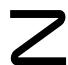
\includegraphics[keepaspectratio]{images/part001_653588be.jpg}}

\begin{enumerate}
\def\labelenumi{\arabic{enumi})}
\setcounter{enumi}{1}
\tightlist
\item
  Let A be a commutative ring. The set of nilpotent elements \(a\) of A is an ideal \(\mathfrak{N}(\mathrm{A})\) of A, called the nilradical of A; it is the intersection of the prime ideals of A (V, §15, No.~1, p.~118, Proposition 2). We have \(\mathfrak{N}(A) \subset \mathfrak{R}(A)\) ; *we have equality if A is an Artinian ring (VIII, p.~173, Corollary 2) or a finitely generated commutative algebra over a commutative field (Comm. Alg., V, §3, n°4, Theorem 3)*. We can certainly have \(\mathfrak{N}(A) \neq \mathfrak{R}(A)\) . This is the case when A is the ring K{[}{[}X{]}{]}, where K is a commutative field: we then have \(\mathfrak{N}(A) = 0\) and \(\mathfrak{R}(A) = AX\) (VIII, p.~154, Example 2).
\end{enumerate}

\subsection{Nakayama's Lemma}

PROPOSITION 6. --- For every A-module M, we have \(\Re(A)M \subset \Re(M)\) . We have equality if the A-module M is projective.

Let P be a maximal submodule of M; the A-module M/P is simple, hence annihilated by \(\Re(\mathrm{A})\) by Proposition 5 of VIII, p.~155. We therefore have \(\Re(\mathrm{A})\mathrm{M}\subset\mathrm{P}\) for every maximal submodule P of M, hence \(\Re(\mathrm{A})\mathrm{M}\subset\Re(\mathrm{M})\) .

We clearly have \(\mathfrak{R}(A_{s})=\mathfrak{R}(A)A_{s}\) . If the A-module M is projective, then there exists an A-module N such that \(M\oplus N\) is free, that is, the direct sum of a family \((\mathrm{L}_{i})_{i\in\mathrm{I}}\) of modules isomorphic to \(A_{s}\) . By Corollary 2 of VIII, p.~152, we have \(\mathfrak{R}(M\oplus N)=\mathfrak{R}(M)\oplus\mathfrak{R}(N)\) and \(\mathfrak{R}\big(\bigoplus_{i\in I}L_{i}\big)=\bigoplus_{i\in I}\mathfrak{R}(L_{i})\) . We then deduce \(\mathfrak{R}(M)=\mathfrak{R}(A)M\) from the equality \(\mathfrak{R}(L_{i})=\mathfrak{R}(A)L_{i}\) .

THEOREM 2 (``Nakayama's lemma''). --- Let M be an A-module and a two-sided ideal of A. Suppose that one of the following conditions is satisfied:

\begin{enumerate}
\def\labelenumi{(\roman{enumi})}
\item
  The A-module M is finitely generated, and \(\mathfrak{a}\) is contained in the radical of A.
\item
  The ideal \(\mathfrak{a}\) is nilpotent.
\end{enumerate}

If N is a submodule of M such that \(M = N + aM\) , then we have N = M. In particular, if the module M is nonzero, then we have \(M \neq aM\) .

Suppose that M is finitely generated and that we have \(\mathfrak{a} \subset \Re(\mathrm{A})\) . Let N be a submodule of M such that \(M = N + aM\) . By Proposition 6, we have \(M = N + \Re(M)\) , hence M = N by Proposition 2, b) of VIII, p.~153.

Now suppose that a is nilpotent, and let N be a submodule of M such that \(M = N + aM\) . By induction on the integer \(n \geqslant 0\) , we establish the relation \(M = N + a^{n}M\) . By assumption, there exists an integer \(n \geqslant 0\) such that \(a^{n} = 0\) ; hence M = N.

The last assertion of the theorem follows from the above by taking N to be 0.

COROLLARY 1. --- We keep the assumptions of Theorem 2. Let \((x_{i})_{i\in\mathrm{I}}\) be a family of elements of M, and let \(\overline{x}_{i}\) be the canonical image of \(x_{i}\) in M/aM. If the family \((\overline{x}_{i})_{i\in\mathrm{I}}\) generates the (A/a)-module M/aM, then the family \((x_{i})_{i\in\mathrm{I}}\) generates the A-module M.

This follows from Theorem 2 applied to the submodule N of M generated by the family \((x_{i})_{i\in \mathbf{I}}\) .

COROLLARY 2. --- We keep the assumptions of Theorem 2. Furthermore, let M' be an A-module and u : M' → M be a homomorphism. If the homomorphism \(\overline{u}\) from M'/aM' to M/aM deduced from u by passing to the quotients is surjective, then u is surjective.

It suffices to apply Theorem 2 to the image N of u: indeed, the image of \(\overline{u}\) is \((\mathrm{N} + \mathfrak{aM})/\mathfrak{aM}\) , so \(\overline{u}\) is surjective if and only if we have \(N + aM = M\) .

\subsection{Lifts of Idempotents}

Lemma 1. --- Let a be an element of a ring A such that \(a - a^{2}\) is nilpotent. There exists a polynomial P in \(\mathrm{X} + (\mathrm{X} - \mathrm{X}^{2})\mathbf{Z}[\mathrm{X}]\) such that \(\mathrm{P}(a)\) is idempotent in A.

Let n be a strictly positive integer such that \((a - a^{2})^{n} = 0\) . Set \(\mathrm{P}(\mathrm{X}) = 1 - (1 - \mathrm{X}^{n})^{n}\) . The polynomial \(\mathrm{P}(\mathrm{X})\) is a multiple of \(X^{n}\) , and the polynomial \(1 - \mathrm{P}(\mathrm{X})\) is a multiple of \((1 - \mathrm{X})^{n}\) , so \(\mathrm{P}(\mathrm{X}) - \mathrm{P}(\mathrm{X})^{2}\) is a multiple of \((\mathrm{X} - \mathrm{X}^{2})^{n}\) , and we have \(\mathrm{P}(a) = \mathrm{P}(a)^{2}\) . Moreover, \(\mathrm{X} - \mathrm{P}(\mathrm{X})\) is a multiple of X and 1 - X, hence a multiple of \(X - X^{2}\) .

PROPOSITION 7. --- Let a be a two-sided nil ideal of A, and let \(\overline{e}\) be an idempotent in the ring A/a. There exists an idempotent e in A whose canonical image in A/a is equal to \(\overline{e}\) .

Let \(a\) be an arbitrary representative of \(\overline{e}\) in \(\mathbf{A}\) . The element \(a - a^2\) of \(\mathbf{A}\) is nilpotent because it belongs to \(\mathfrak{a}\) . Choose a polynomial \(\mathrm{P} \in \mathbf{Z}[\mathrm{X}]\) satisfying the conditions of Lemma 1. We have \(a - \mathrm{P}(a) \in \mathrm{A}(a - a^2)\) , so the element \(e = \mathrm{P}(a)\) of \(\mathbf{A}\) has the desired property.

\pandocbounded{
\includegraphics[keepaspectratio]{images/part001_2ad691f6.jpg}}

Suppose that \(\bar{e}\) belongs to the center of the ring A/a. There does not necessarily exist an idempotent e in the center Z of A lifting \(\bar{e}\) (VIII, p.~172, Exercise 31). However, if \(\bar{e}\) belongs to the image of Z in A/a, then it lifts to an idempotent in Z because \(Z \cap a\) is a nil ideal of Z.

COROLLARY 1. --- Let M and P be A-modules and u a surjective A-linear mapping from P to M. Suppose that P is projective and that there exists a nilpotent two-sided ideal \(\mathfrak{a}\) of A such that the kernel N of \(u\) is contained in \(\mathfrak{aP}\) . Let \(\mathrm{M}'\) and \(\mathrm{M}''\) be submodules of M whose direct sum is M. Then P is the direct sum of submodules \(\mathrm{P}'\) and \(\mathrm{P}''\) such that \(u(\mathrm{P}') = \mathrm{M}'\) and \(u(\mathrm{P}''') = \mathrm{M}''\) .

Denote by B the subring of \(\operatorname{End}_{\mathrm{A}}(\mathrm{P})\) consisting of the endomorphisms f of P such that \(f(\mathrm{N}) \subset \mathrm{N}\) . Let \(\overline{B}\) be the endomorphism ring of M. For \(f \in B\) , let \(\overline{f}\) be the unique endomorphism of M such that \(\overline{f} \circ u = u \circ f\) . The mapping \(f \mapsto \overline{f}\) is a ring homomorphism from B to \(\overline{B}\) . Since the module P is projective, this homomorphism is surjective; its kernel b consists of the endomorphisms \(f \in B\) such that \(f(\mathrm{P}) \subset \mathrm{N}\) . Let n be a natural number such that \(a^{n} = 0\) . We have

\[
\mathrm{P} = \mathfrak {a} ^ {0} \mathrm{P} \supset \mathfrak {a} ^ {1} \mathrm{P} \supset \dots \supset \mathfrak {a} ^ {n - 1} \mathrm{P} \supset \mathfrak {a} ^ {n} \mathrm{P} = 0,
\]

and, for every \(f \in b\) and every integer \(j \geqslant 0\) ,

\[
f (\mathfrak {a} ^ {j} \mathrm{P}) = \mathfrak {a} ^ {j} f (\mathrm{P}) \subset \mathfrak {a} ^ {j} \mathrm{N} \subset \mathfrak {a} ^ {j + 1} \mathrm{P}
\]

because \(N \subset aP\) by assumption. We therefore have \(f(P) \subset a^{j}P\) for every natural number j and every \(f \in b^{j}\) . In particular, we have \(b^{n} = 0\) .

Let \(\varepsilon'\) be the projector of M with image M' and kernel M'\,`. By Proposition 7 applied to the ring B and the nilpotent two-sided ideal b, there exists an idempotent \(e'\) in B such that \(\overline{e'} = \varepsilon'\) , that is, \(\varepsilon' \circ u = u \circ e'\) . Set \(e'' = 1 - e'\) , \(\varepsilon'' = \overline{e''}\) , P' = \(e'(P)\) , and P'\,' = \(e''(P)\) . Then P is the direct sum of the submodules P' and P'\,', and we have

\[
u (\mathrm{P} ^ {\prime}) = u (e ^ {\prime} (\mathrm{P})) = \varepsilon^ {\prime} (u (\mathrm{P})) = \varepsilon^ {\prime} (\mathrm{M}) = \mathrm{M} ^ {\prime};
\]

the equality \(u(\mathrm{P}'') = \mathrm{M}''\) is proved analogously.

COROLLARY 2. --- Let A be a ring, and let a be a nilpotent two-sided ideal of A. If P is a projective A-module, then P/aP is a projective module over A/a, and the A-module P is indecomposable if and only if the A/a-module P/aP is indecomposable.

Let P be a projective A-module, and let \(\overline{P}\) be the A/a-module P/aP. The A-module P is zero if and only if \(\overline{P}\) is zero (Theorem 2 of VIII, p.~158). Now suppose \(P \neq 0\) . Since the A/a-module \(\overline{P}\) is isomorphic to \(\overline{A} \otimes_{A} P\) , it is projective (II, §5, No.~1, p.~279, Corollary of Proposition 4). If P is indecomposable, then so is \(\overline{P}\) by Corollary 1. Conversely, suppose that P is decomposable and nonzero, and let \(P'\) and \(P''\) be two nonzero submodules of P such that \(P = P' \oplus P''\) . By Nakayama's lemma (VIII, p.~158, Theorem 2), we have \(P' + aP \neq P\) and \(P'' + aP \neq P\) ; if \(\overline{P}'\) and \(\overline{P}''\) are the canonical images of \(P'\) and \(P''\) in \(\overline{P}\) , then we have \(\overline{P}' \neq \overline{P}\) , \(\overline{P}'' \neq \overline{P}\) , and \(\overline{P} = \overline{P}' \oplus \overline{P}''\) . This proves that \(\overline{P}\) is decomposable.
